\documentclass[a4paper,11pt]{article}
\usepackage[english,greek]{babel}
\usepackage[utf8]{inputenc}
\usepackage[T1]{fontenc}
\usepackage{textcomp}

\usepackage{amsmath, amsthm, amssymb}
\usepackage{bm}

\usepackage{libertine}

\usepackage{url}
\usepackage{hyperref}
\hypersetup{
    unicode=true,
    pdftitle={Geometrical Control Theory problem set 2},
    pdfauthor={Vasilas Nikos},
    pdfsubject={Geometrical Control Theory},
    pdfcreator={Vasilas Nikos},
    pdfproducer={Vasilas Nikos},
    pdfkeywords={control, nonlinear, math},
}

\usepackage{graphicx}
\usepackage[small,bf]{caption}
\usepackage{subcaption}

\usepackage{booktabs}

\usepackage
[a4paper, top=1.0in, bottom=1.25in, left=1.25in, right=1.25in]{geometry}
\headsep=20pt
\footskip=30pt

\usepackage{authoraftertitle}

\makeatletter
\renewcommand{\maketitle}{\bgroup\setlength{\parindent}{0pt}
\thispagestyle{plain}
\begin{flushleft}
    \textbf{\Huge{\@title}\\}
    \vspace{2em}
    \@author
    \vspace{2em}
\end{flushleft}\egroup
}
\makeatother

\usepackage{csquotes}
%\usepackage[backend=biber, bibencoding=auto, autolang=other]{biblatex}
%\addbibresource{bible.bib}

\newcommand{\tl}[1]{\textlatin{#1}}
\newcommand{\gr}[1]{\greektext{#1}}
\newcommand{\greek}{\selectlanguage{greek}}
\newcommand{\eng}{\selectlanguage{english}}

\usepackage{enumitem}
\newenvironment{alphenum}
{\begin{enumerate}
    [itemsep=-0.5ex, topsep=1.0ex, leftmargin=\parindent, align=left,
    labelwidth=!, label=\((\alph*)\)]}
{\end{enumerate}}

\newenvironment{romenum}
{\begin{enumerate}
    [itemsep=-5pt, leftmargin=*, labelsep=1em, align=left, labelwidth=!,label=\((\roman*)\)]}
{\end{enumerate}}

\usepackage{mathtools}
\newcommand\defeq{\coloneq}
\newcommand\eqdef{\eqcolon}

\newcommand\proofpt[1]{\({(#1)}\)}

\newcommand\inner[2]{\langle#1,\, #2\rangle}

\newcommand\dual[1]{#1^{*}}
\newcommand\algdual[1]{#1^{\#}}

\newcommand\lmaps{\mathcal{B}}

\newcommand\realf{R}
\newcommand\euclr[1]{\realf^{#1}}
\newcommand\deuclr[1]{\dual{(\euclr{#1})}}

\newcommand\restr[2]{#1|_#2}
\newcommand\compf{\mathbb{C}}
\newcommand\matrx[1]{\mathrm{#1}}
\newcommand\pcmap[1]{PC^{#1}}
\newcommand\cdiff[1]{C^{#1}}
\newcommand\metric{d}
\newcommand\di[2]{\metric(#1, #2)}

\newcommand{\vc}[1]{\bm{#1}} % this is a vector
\newcommand{\mt}[1]{\boldsymbol{#1}} % this is a matrix

\DeclareMathOperator\rank{rank}
\DeclareMathOperator\vspan{span}
\DeclareMathOperator\co{co}
\DeclareMathOperator\aff{aff}
\DeclareMathOperator\core{cor}
\DeclareMathOperator\icr{icr}
\DeclareMathOperator\diag{diag}
\DeclareMathOperator\minimize{minimize}
\DeclareMathOperator\argmin{arg\,min}
\DeclareMathOperator\der{D}
\DeclareMathOperator\qi{qi}
\DeclareMathOperator\qci{qci}
\DeclareMathOperator{\tr}{tr}

\newcommand\cseg[2]{[#1, #2]}
\newcommand\sseg[2]{[#1, #2)}
\newcommand\oseg[2]{(#1, #2)}

\newcommand\eps{\varepsilon}
\newcommand\dsum{\oplus}

\newcommand\norm[2][{}]{\|#2\|_{#1}}

\makeatletter
\newcommand\suchthat{%
    \@ifstar
    {\mathrel{}\middle|\mathrel{}}
    {\mid}%
}
\makeatother
\makeatletter
\newcommand\setbuild[2]{
    \@ifstar
    {\left\{#1\suchthat* #2\right\}}%
    {\{#1\suchthat #2\}}%
}
\makeatother
\newcommand\ball[2]{B_{#1}(#2)}
\newcommand\cball[2]{\closure{B}_{#1}(#2)}
\newcommand\oball[1]{B_{#1}}
\newcommand\ocball[1]{\bar{B}_{#1}}
\newcommand\compl[1]{#1^{\mathrm{c}}}
\newcommand\closure[2][.0]
{
    \mkern#1mu
    \overline{\mkern-#1mu#2}
}
\newcommand\interior[1]{{#1}^{\circ}}
\newcommand\boundary[1]{\partial#1}
\newcommand\voidset{\varnothing}

\newcommand\nulls[1]{\mathcal{N}(#1)}
\newcommand\range[1]{\mathcal{R}(#1)}

\newcommand\refthrm[2][]{Theorem \ifx\\#1\\\ref{#2}\else\ref{#2} \ref{#1}\fi}
\newcommand\refprop[2][]{Proposition \ifx\\#1\\\ref{#2}\else\ref{#2} \ref{#1}\fi}
\newcommand\reflemma[2][]{Lemma \ifx\\#1\\\ref{#2}\else\ref{#2} \ref{#1}\fi}

\renewcommand\theequation{\arabic{equation}}
\newtheoremstyle{thrm_style}
{} %spaceabove
{} %spacebelow
{\itshape} %bodyfont
{} %indent
{\bfseries} %headfont
{} %headpunctuation
{1em} %headspace
{\thmnumber{#2\kern1em}\thmname{#1}\thmnote{ (#3)}} %headspec
\theoremstyle{thrm_style}
\newtheorem{thrm}{\gr{Θεώρημα}}
\newtheorem{prop}[thrm]{\gr{Πρόταση}}
\newtheorem{cor}[thrm]{\gr{Πόρισμα}}
\newtheorem{lemma}[thrm]{\gr{Λήμμα}}

\newcommand\theoremname{}
\newtheorem{genericthrm}[thrm]{\theoremname}
\newenvironment{namedthrm}[1]
{\renewcommand\theoremname{#1}
\begin{genericthrm}}
{\end{genericthrm}}

\newtheoremstyle{defn_style}
{} %spaceabove
{} %spacebelow
{} %bodyfont
{} %indent
{\bfseries} %headfont
{} %headpunctuation
{1em} %headspace
{\thmnumber{#2\kern1em}\thmname{#1}\thmnote{ (#3)}} %headspec
\theoremstyle{defn_style}
\newtheorem{defn}[thrm]{\gr{Ορισμός}}
\newtheorem{exmp}[thrm]{\gr{Παράδειγμα}}

\newcommand\defnname{}
\newtheorem{genericdefn}[thrm]{\defnname}
\newenvironment{nameddefn}[1]
{\renewcommand\defnname{#1}
\begin{genericdefn}}
{\end{genericdefn}}

\newtheoremstyle{rem_style}
{} %spaceabove
{} %spacebelow
{} %bodyfont
{} %indent
{\bfseries} %headfont
{.} %headpunctuation
{.5em} %headspace
{\thmnumber{#2\kern1em}\thmname{#1}\thmnote{ (#3)}} %headspec
\theoremstyle{rem_style}
\newtheorem*{rem}{Remark}
\newtheorem*{note}{Note}

\renewcommand\qed{\unskip\nobreak\quad\qedsymbol}
\renewcommand\qedsymbol{\rule{1ex}{1.6ex}}

\newenvironment{exercise}[2][Άσκηση]
{\begin{trivlist}
    \item[\hskip \labelsep {\bfseries #1}\hskip \labelsep {\bfseries #2.}]}
{\end{trivlist}}

\newenvironment{solution}[1][Λύση]
{\begin{trivlist}
    \item[\hskip \labelsep {\bfseries #1}]}
{\end{trivlist}}


\iffalse
    \begin{figure}[h]
        \centering
        \begin{subfigure}[b]{0.55\textwidth}
            \includegraphics[width=\textwidth]{figures/undampedPend.eps}
        \end{subfigure}
        \begin{subfigure}[b]{0.55\textwidth}
            \includegraphics[width=\textwidth]{figures/undampedPendVec.eps}
        \end{subfigure}
        \caption{\gr{Πορτρέτο κίνησης και διανυσματικό πεδίο}}
    \end{figure}
\fi
\begin{document}
\title{Γεωμετρική Θεωρία Ελέγχου}
\author{2\textsuperscript{η} Σειρά Ασκήσεων\\Βασίλας Νικόλαος}
\maketitle

\begin{exercise}{2016/17 1}
    Βρείτε δύο διαφορετικά παραδείγματα συστημάτων στο επίπεδο με σημείο
    ισορροπίας στο \( (0, 0) \) το οποίο ενώ έχει γειτονιά \( N_{\epsilon}(0) \)
    τέτοια ώστε \( x \in N_{\epsilon}(0) \Rightarrow \lim_{t \to \infty} \phi(x,
    t) = 0 \), δεν είναι ευσταθές κατά \tl{Lyapunov}. Εξηγήστε γιατί τέτοια
    παραδείγματα είναι κατ᾽ ανάγκην μη-γραμμικά.
\end{exercise}
\begin{solution}{2016/17 1}
    Το σημείο \( \bar{x} \) είναι ευσταθές σημείο ισορροπίας αν για κάθε
    γειτονιά \( U \) του \( \bar{x} \), υπάρχει γειτονιά \( U_1 \) του
    \( \bar{x} \) τέτοια ώστε κάθε λύση \( x(t) \) με \( x(0) \) στο \( U_1 \),
    να υπάρχει και να ορίζεται στο \( U \) για κάθε \( t > 0 \). Αν το \( U_1 \)
    μπορεί να επιλεχθεί έχοντας τις ιδιότητες που περιγράφηκαν και ακόμα ισχύει
    \( \lim_{t \to \infty} x(t) = \bar{x} \), τότε το \( \bar{x} \) είναι
    ασυμπτωτικά ευσταθές. Στην άσκηση μας δίνεται ότι η λύση είναι
    συγκλίνουσα στο \( 0 \) και μας δίνεται μία γειτονιά του \( 0 \) που
    οι λύσεις είναι συγκλίνουσες. Αυτό όμως δεν προϋποθέτει ότι το σημείο
    είναι ευσταθές στη γενική περίπτωση, καθώς τίποτα δε μας διασφαλίζει ότι
    για κάθε \( U \), που θα φράζει τη \( x(t) \), θα μπορούμε να βρούμε λύσεις
    που ξεκινούν στη \( N_{\epsilon}(0) \) και θα παραμένουν εντός του συνόλου
    \( U \). Συνεπώς, μπορούμε κάλλιστα να έχουμε μία συμπεριφορά όπως
    αυτή που απεικονίζεται στο σχήμα~\ref{fig:ex1_unstable_convergent}.
    \begin{figure}[h]
        \centering
        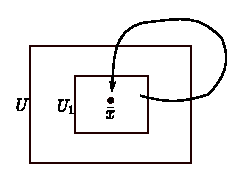
\includegraphics[width=0.4\textwidth]{figures/ex1_unstable_convergent.eps}
        \caption{\gr{Ασταθές, συγκλίνων σημείο.}}
        \label{fig:ex1_unstable_convergent}
    \end{figure}

    Ένα παράδειγμα που παρουσιάζει αυτή τη συγκλίνουσα αλλά ασταθή συμπεριφορά
    είναι το παρακάτω.
    \begin{align*}
        \dot{x}_1 &= x_1^2 - x_2^2 \\
        \dot{x}_2 &= 2x_1^2x_2^2.
    \end{align*}
    Το σημείο ισορροπίας του συστήματος είναι το \( (0, 0) \). Κάθε τροχιά του
    συστήματος τείνει στην αρχή των αξόνων καθώς \( t \to \infty \), εκτός από
    τις τροχιές που ξεκινούν στον άξονα \( x_1 \), οι οποίες παραμένουν εκεί για
    κάθε χρόνο. Στο σχήμα~\ref{fig:ex1_unstable_convergent_example} βλέπουμε το
    διάγραμμα του διανυσματικού πεδίου για το παράδειγμά μας.
    \begin{figure}[h]
        \centering
        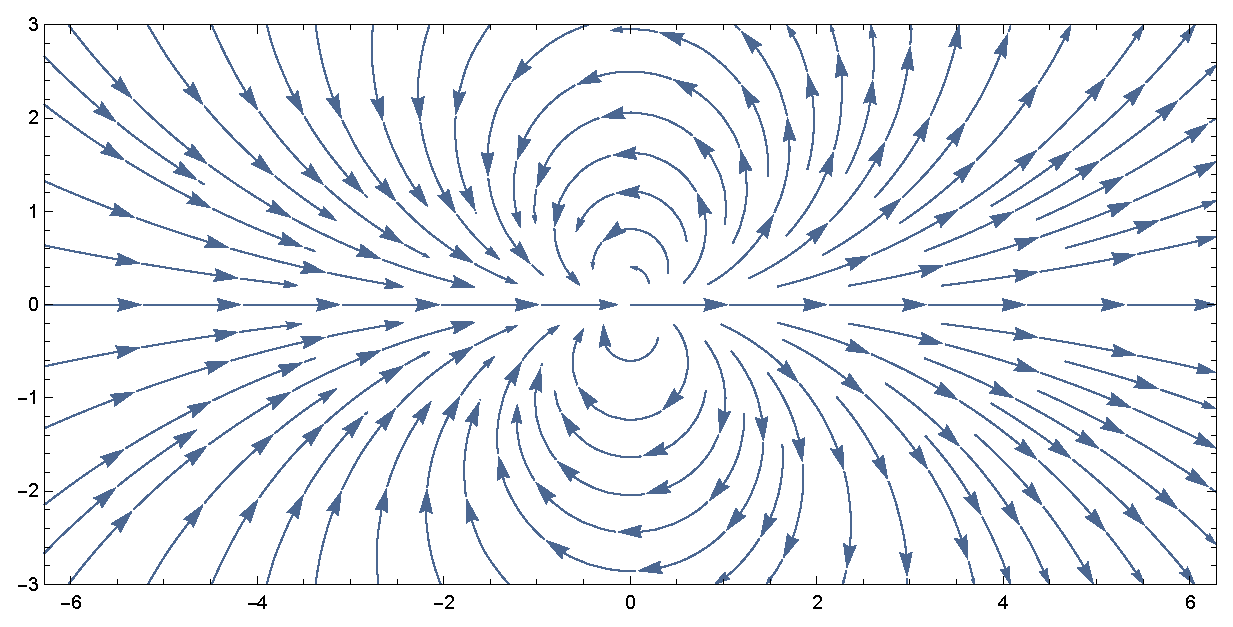
\includegraphics[width=1\textwidth]{figures/ex1_unstableConvergentExample.eps}
        \caption{\gr{Παράδειγμα ασταθούς, συγκλίνουν σημείου.}}
        \label{fig:ex1_unstable_convergent_example}
    \end{figure}

    Τέτοια παραδείγματα είναι κατ᾽ ανάγκην μη-γραμμικά. Η ευστάθεια ενός
    γραμμικού συστήματος της μορφής
    \begin{equation*}
        \dot{x}(t) = Ax(t), \quad x(0) = x_0,
    \end{equation*}
    εξαρτάται αποκλειστικά και μόνο από τη φασματική δομή του πίνακα \( A \).
    Επίσης, το σύστημα έχει τη γνωστή λύση
    \begin{equation*}
        x(t) = e^{At}x_0.
    \end{equation*}
    Επομένως, ο μόνος τρόπος ώστε η παραπάνω να ικανοποιεί το \( \lim_{t \to
    \infty} \phi(x, t) \) είναι οι ιδιοτιμές του πίνακα \( A \) να έχουν
    αρνητικό πραγματικό μέρος. Αυτό εύκολα φαίνεται αν πάρουμε τη μορφή
    \tl{Jordan} του πίνακα \( A \), έτσι στη διαγώνιο θα έχουμε τις ιδιοτιμές
    και το ζητούμενο όριο θα ικανοποιείται μόνο όταν είναι αρνητικές. Αυτό
    σημαίνει ότι, για τα γραμμικά συστήματα αν ικανοποιείται το όριο τότε αυτό
    σημαίνει και ασυμπτωτική ευστάθεια.
\end{solution}

\begin{exercise}{2016/17 2}
    \emph{Το σύστημα του \tl{Duffing}}: Το σύστημα
    \begin{align*}
        \dot{x} &= y \\
        \dot{y} &= -\zeta y + x - x^3, \quad \zeta \geq 0
    \end{align*}
    στο επίπεδο είναι η κανονική μορφή της αυτόνομης Δ.Ε.
    \begin{equation*}
        \ddot{x} + \zeta\dot{x} + x^3 - x = 0.
    \end{equation*}
    περιγράφει ένα σύστημα με απόσβεση που κινείται σε συμμετρικό δυναμικό με
    δύο ελάχιστα (γιατί;)
    \begin{enumerate}[label = (\alph*)]
        \item Θα μελετήσουμε πρώτα την περίπτωση \( \zeta = 0 \). Το σύστημα
            είναι συντηρητικό (Χαμιλτονιανό), της μορφής \( \dot{x} = y, \dot{y}
            = - \nabla U(x) \). Επαληθεύστε ότι ισχύει αυτό, δώστε την
            Χαμιλτονιανή συνάρτηση \( H(x, y) \) και το διάγραμμα ροής (πορτρέτο
            κίνησης ή φάσεων).
        \item Τώρα περνάμε στην περίπτωση \( \zeta > 0 \). Βρείτε τα σημεία
            ισορροπίας και την (τοπική) τους συμπεριφορά. Δείξτε ότι, κατάλληλα
            μετατοπισμένη, η \( H \) είναι συνάρτηση \tl{Lyapunov} και εξηγήστε
            γιατί αποτελεί υποσύνολο της περιοχής έλξης κάθε Σ.Ι. Δείξτε ότι εάν
            \emph{τρέξουμε} τα σύνολα αυτά προς τα πίσω (σε αρνητικό χρόνο) θα
            πάρουμε τη συνολική έλξης. Προσπαθήστε να δώσετε ένα διάγραμμα των
            περιοχών αυτών για διάφορες τιμές του \( \zeta \). Πόσες
            καμπύλες/τροχιές αποτελούν το διαχωριστικό σύνολο των δύο περιοχών
            έλξης;
    \end{enumerate}
\end{exercise}
\begin{solution}{2016/17 2}
    1. Οι εξισώσεις του συστήματος χωρίς απόσβεση είναι
    \begin{align*}
        \dot{x} &= y \\
        \dot{y} &= x - x^3.
    \end{align*}
    Τα σημεία ισορροπίας υπολογίζονται από τις σχέσεις
    \begin{align*}
        0 &= y \\
        0 &= x - x^3,
    \end{align*}
    και από τη δεύτερη σχέση έχουμε
    \begin{equation*}
        x(1 - x^2) = 0,
    \end{equation*}
    που σημαίνει \( x = 0 \) ή \( x = \pm 1 \). Άρα έχουμε τα σημεία
    ισορροπίας είναι \( (0, 0), (1, 0), (-1, 0) \).

    Επειδή δεν έχουμε απόσβεση, έχουμε Χαμιλτονιανό δυναμικό σύστημα με
    \( q = x, p = y \) και θέλουμε
    \begin{equation*}
        \frac{\partial H}{\partial y} = y, \quad
        \frac{\partial H}{\partial x} = -x + x^3.
    \end{equation*}
    Έτσι θέλουμε
    \begin{equation}\label{eq:ex2_hamiltonian}
        H(x, y) = \frac{1}{2}y^2 + U(x),
    \end{equation}
    με συνάρτηση δυναμικού
    \begin{align}\label{eq:ex2_potential}
        U(x) &= - \int_0^x \left(\bar{x} - \bar{x}^3 \right) \, d\bar{x}
        \nonumber \\
        &= -\frac{1}{2}x^2 + \frac{1}{4}x^4.
    \end{align}
    Μάλιστα μπορούμε να επιβεβαιώσουμε ότι είναι Χαμιλτονιανό καθώς έχουμε
    \begin{align*}
        \frac{dH}{dt}
        &= y\dot{y} - x\dot{x} + x^3\dot{x} \\
        &= y(x - x^3) - xy + x^3y = 0.
    \end{align*}
    Συνεπώς, το σύστημα είναι της μορφής
    \begin{align*}
        \dot{x} &= y \\
        \dot{y} &= -\nabla U(x) = -\nabla\left( -\frac{1}{2}x^2 +
        \frac{1}{4}x^4 \right),
    \end{align*}
    ή τελικά
    \begin{align*}
        \dot{x} &= y \\
        \dot{y} &= x - x^3.
    \end{align*}
    Από τη σχέση~\eqref{eq:ex2_hamiltonian}, διαπιστώνουμε ότι οι λύσεις του
    συστήματος, είναι συμμετρικές ως προς τον άξονα των τετμημένων, καθώς
    η συνολική ενέργεια \( H(x, y) \) είναι σταθερή. Έτσι κάθε λύση ή τροχιά
    ανήκει σε μία ισοϋψή καμπύλη που εξαρτάται από την αρχική ενέργεια
    \( h_0 \). Έτσι οι λύσεις είναι
    \begin{equation*}
        y = \pm \sqrt{2h_0 + x^2 - \frac{1}{2}x^4}.
    \end{equation*}
    Η κλίση των τροχιών στο επίπεδο φάσεων είναι
    \begin{equation*}
        \frac{dy}{dx} = \frac{x - x^3}{y}.
    \end{equation*}
    Από τη σχέση της συνάρτησης δυναμικού~\eqref{eq:ex2_potential} καθώς από
    την παραπάνω σχέση φαίνεται ότι η συνάρτηση δυναμικού παρουσιάζει ακρότατο
    στα σημεία ισορροπίας. Αυτό συμβαίνει διότι εκεί ισχύει
    \begin{align*}
        0 &= U'(x) \\
        &= x^3 - x,
    \end{align*}
    και έτσι επιβεβαιώνεται ότι τα κρίσιμα σημεία της συνάρτησης είναι τα
    \( 0, \pm 1 \).

    Για να χαρακτηρίσουμε τα σημεία ισορροπίας, γράφουμε τις εξισώσεις που
    διέπουν το σύστημα στη μορφή
    \begin{equation*}
        \begin{pmatrix}
            \dot{x} \\
            \dot{y}
        \end{pmatrix} = F(x, y) =
        \begin{pmatrix}
            y \\
            x - x^3
        \end{pmatrix}.
    \end{equation*}
    Αν πάρουμε τη γραμμικοποίηση, θα έχουμε
    \begin{equation*}
        DF(x, y) =
        \begin{pmatrix}
            0 & 1 \\
            1 - 3x^2 & 0
        \end{pmatrix}.
    \end{equation*}

    Για το σημείο ισορροπίας \( (0, 0) \) ισχύει
    \begin{equation*}
        DF(0, 0) =
        \begin{pmatrix}
            0 & 1 \\
            1 & 0
        \end{pmatrix}
    \end{equation*}
    που συνεπάγεται
    \begin{equation*}
        \lambda_1 = 1, \quad \lambda_2 = -1.
    \end{equation*}
    Από το θεώρημα \tl{Hartman–Grobman}, επειδή το σημείο είναι
    υπερβολικό, και επειδή έχουμε σάγμα στο \( (0, 0) \) στο γραμμικοποιημένο
    σύστημα, θα έχουμε σάγμα στο \( (0, 0) \) και για το αρχικό μη-γραμμικό
    σύστημα.

    Με αντίστοιχη διαδικασία, για το σημείο ισορροπίας \( (1, 0) \) ισχύει
    \begin{equation*}
        DF(1, 0) =
        \begin{pmatrix}
            0 & 1 \\
            -2 & 0
        \end{pmatrix}
    \end{equation*}
    που συνεπάγεται
    \begin{equation*}
        \lambda = \pm i\sqrt{2}.
    \end{equation*}
    Στην περίπτωση αυτή, έχουμε φανταστικές ιδιοτιμές και έτσι δεν μπορούμε να
    βγάλουμε κάποιο συμπέρασμα από το θεώρημα \tl{Hartman-Grobman}. Παρόλο αυτά
    έχουμε συμπεριφορά κέντρου στο \( (1, 0) \) για το γραμμικοποιημένο σύστημα.

    Στο ίδιο αποτέλεσμα καταλήγουμε και για το σημείο ισορροπίας \( (-1,
    0) \), καθώς ο όρος που σχετίζεται με τη μεταβλητή \(x\) στον πίνακα
    γραμμικοποίησης είναι τετραγωνικός.

    Η ακριβής φύση των κρίσιμων σημείων, μπορεί να καθοριστεί από τη συνάρτηση δυναμικού
    και από την τιμή της δεύτερης παραγώγου στα σημεία αυτά. Έτσι
    \begin{equation*}
        U''(x) = 3x^2 - 1.
    \end{equation*}
    Στα σημεία \( 1 \) και \( -1 \), η συνάρτηση δυναμικού παρουσιάζει τοπικό
    ελάχιστο, \( U''(1) = U''(-1) = 2 > 0 \), ενώ στο σάγμα \( U''(0) = -1 < 0
    \) τοπικό μέγιστο.

    \begin{figure}[h]
        \centering
        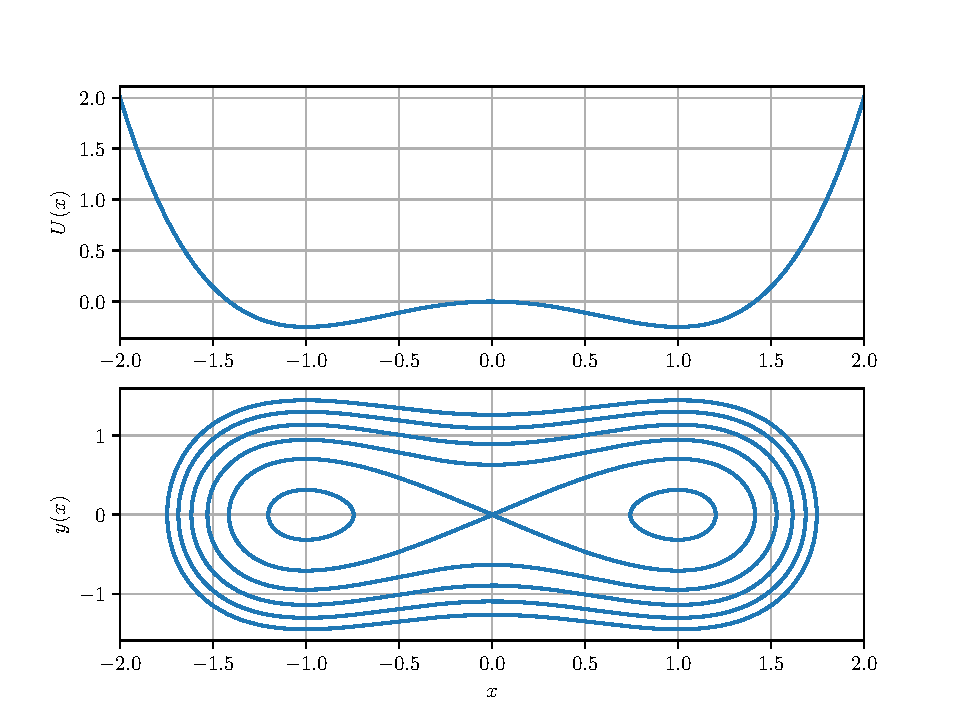
\includegraphics[width=1\textwidth]{figures/ex2_undampedDuffing.pdf}
        \caption{\gr{Συνάρτηση δυναμικού και ταλαντωτής \tl{Duffing} χωρίς απόσβεση.}}
        \label{fig:ex2_undampedDuffing}
    \end{figure}
    \begin{figure}[h]
        \centering
        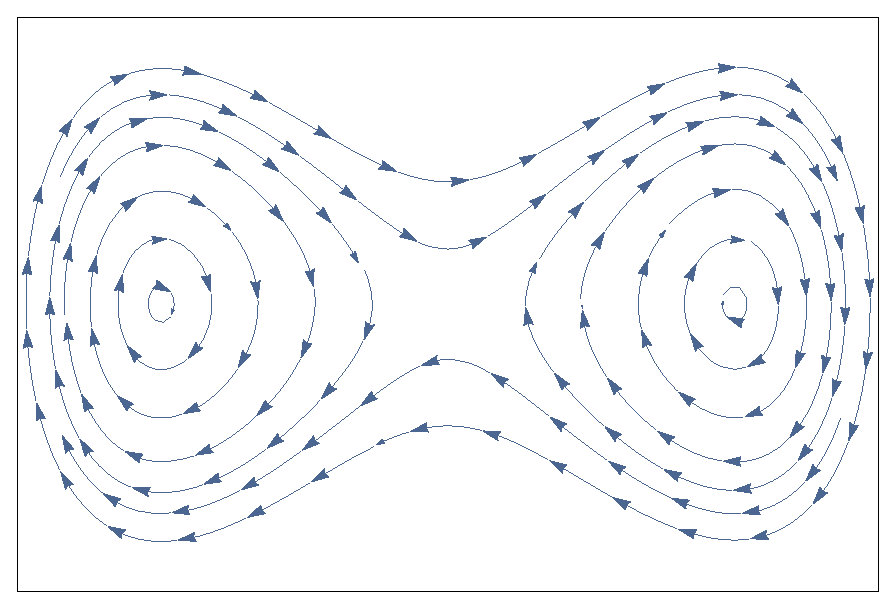
\includegraphics[width=0.8\textwidth]{figures/ex2_undampedDuffingVectorField.eps}
        \caption{\gr{Πορτρέτο κίνησης ταλαντωτή \tl{Duffing} χωρίς απόσβεση.}}
        \label{fig:ex2_undampedDuffingVectorField}
    \end{figure}
    Στο επάνω σχήμα της~\ref{fig:ex2_undampedDuffing} βλέπουμε τη συνάρτηση
    δυναμικού και στο κάτω το πορτρέτο φάσεων του ταλαντωτή \tl{Duffing} χωρίς
    απόσβεση. Όπως παρατηρούμε, η συνάρτηση δυναμικού παρουσιάζει τα ακρότατα
    στα σημεία ισορροπίας. Στα σημεία \( (-1, 0) \) και \( (1, 0) \) παρατηρούμε
    ότι έχουμε συμπεριφορά κέντρου, και στο σημείο \( (0, 0) \) έχουμε σάγμα.
    Στο σχήμα~\ref{fig:ex2_undampedDuffingVectorField} παρουσιάζεται η
    συμπεριφορά του διανυσματικού πεδίου.

    2. Στην περίπτωση όπου το \( \zeta > 0 \), οι εξισώσεις θα είναι
    \begin{equation*}
        \begin{pmatrix}
            \dot{x} \\
            \dot{y}
        \end{pmatrix} = F(x, y) =
        \begin{pmatrix}
            y \\
            -\zeta y + x - x^3
        \end{pmatrix}.
    \end{equation*}
    Τα σημεία ισορροπίας υπολογίζονται από τις σχέσεις
    \begin{align*}
        0 &= y \\
        0 &= -\zeta y + x - x^3,
    \end{align*}
    και από τη δεύτερη σχέση έχουμε
    \begin{equation*}
        x(1 - x^2) = 0,
    \end{equation*}
    που σημαίνει \( x = 0 \) ή \( x = \pm 1 \), και άρα έχουμε τα σημεία
    ισορροπίας παραμένουν τα ίδια και είναι \( (0, 0), (1, 0), (-1, 0) \).

    Η γραμμικοποίηση, είναι
    \begin{equation*}
        DF(x, y) =
        \begin{pmatrix}
            0 & 1 \\
            1 - 3x^2 & -\zeta
        \end{pmatrix}
    \end{equation*}
    και για το σημείο ισορροπίας \( (0, 0) \) ισχύει
    \begin{equation*}
        DF(0, 0) =
        \begin{pmatrix}
            0 & 1 \\
            1 & -\zeta
        \end{pmatrix}.
    \end{equation*}
    Οι ιδιοτιμές της γραμμικοποίησης στο \( (0, 0) \) είναι
    \begin{equation*}
        \det
        \begin{pmatrix}
            -\lambda & 1 \\
            1 & -\zeta - \lambda
        \end{pmatrix}.
    \end{equation*}
    που σημαίνει ότι
    \begin{equation*}
        \lambda^2 + \zeta \lambda - 1 = 0,
    \end{equation*}
    και μας δίνει τις λύσεις
    \begin{equation*}
        \lambda = \frac{1}{2}\left( -\zeta \pm \sqrt{\zeta^2 + 4} \right).
    \end{equation*}
    Αν συμβολίσουμε με \( \lambda_1 \) την ιδιοτιμή που προκύπτει από το θετικό
    πρόσημο που είναι μπροστά από την τετραγωνική ρίζα και αντίστοιχα με
    \( \lambda_2 \) την άλλη ιδιοτιμή, παρατηρούμε ότι \( \lambda_1 > 0 \).
    Γιατί αν ίσχυε \( \lambda_1 \leq 0 \) τότε
    \begin{align*}
        -\zeta + \sqrt{\zeta^2 + 4} &\leq 0 \\
        \sqrt{\zeta^2 + 4} &\leq \zeta \\
        \zeta^2 + 4 &\leq \zeta^2,
    \end{align*}
    άτοπο. Επίσης, είναι ξεκάθαρο ότι \( \lambda_2 < 0 \) διότι \( \zeta > 0 \)
    και άρα έχουμε σάγμα για τη γραμμικοποίηση. Συνεπώς, από το θεώρημα
    \tl{Hartman–Grobman}, επειδή το σημείο είναι υπερβολικό, θα έχουμε σάγμα στο
    \( (0, 0) \) και για το αρχικό μη-γραμμικό σύστημα.

    Για το σημείο ισορροπίας \( (1, 0) \) ισχύει
    \begin{equation*}
        DF(1, 0) =
        \begin{pmatrix}
            0 & 1 \\
            -2 & -\zeta
        \end{pmatrix}.
    \end{equation*}
    Οι ιδιοτιμές της γραμμικοποίησης στο \( (1, 0) \) είναι
    \begin{equation*}
        \det
        \begin{pmatrix}
            -\lambda & 1 \\
            -2 & -\zeta - \lambda
        \end{pmatrix}.
    \end{equation*}
    που σημαίνει ότι
    \begin{equation*}
        \lambda^2 + \zeta \lambda + 2 = 0,
    \end{equation*}
    και μας δίνει τις λύσεις
    \begin{equation*}
        \lambda = \frac{1}{2}\left( -\zeta \pm \sqrt{\zeta^2 - 8} \right).
    \end{equation*}
    Συμβολίζουμε με \( \lambda_1 \) την ιδιοτιμή με προκύπτει από το θετικό
    πρόσημο που είναι μπροστά από την τετραγωνική ρίζα και αντίστοιχα με
    \( \lambda_2 \) την άλλη ιδιοτιμή. Οι ρίζες της διακρίνουσας είναι \(
    -2\sqrt{2} \) και \( 2\sqrt{2} \). Όμως η απόσβεση είναι αυστηρά θετική και
    έτσι η διακρίνουσα είναι αρνητική για \( \zeta \in (0, 2\sqrt{2}) \) και
    θετική για \( \zeta > 2\sqrt{2} \).

    Στην περίπτωση όπου το \( \zeta \in (0, 2\sqrt{2}) \) τότε επειδή
    το πραγματικό μέρος είναι πάντα αρνητικό, το σημείο ισορροπίας \( (1,
    0) \), από το θεώρημα \tl{Hartman-Grobman}, είναι ασυμπτωτικά ευσταθές
    και έχει τη μορφή ευσταθούς εστίας.

    Στην περίπτωση όπου το \( \zeta > 2\sqrt{2} \) τότε φυσικά η \( \lambda_2 =
    1/2 \left( -\zeta - \sqrt{\zeta^2 - 8} \right) < 0 \), αλλά και η \( \lambda_1 =
    1/2 \left( -\zeta +\sqrt{\zeta^2 - 8} \right) < 0 \). Γιατί αν \( \lambda_1
    \geq 0 \) τότε
    \begin{align*}
        -\zeta + \sqrt{\zeta^2 - 8} &\geq 0 \\
        \zeta^2 - 8 &\geq \zeta^2,
    \end{align*}
    άτοπο.

    Άρα στην περίπτωση όπου το \( \zeta > 2\sqrt{2} \) τότε το σημείο
    ισορροπίας \( (1, 0) \), από το θεώρημα \tl{Hartman-Grobman}, είναι
    ασυμπτωτικά ευσταθές και έχει τη μορφή ευσταθούς κόμβου.

    Τέλος, για \( \zeta = 2\sqrt{2} \) έχουμε διπλή ρίζα και στο σημείο
    ισορροπίας \( (1, 0) \), από το θεώρημα \tl{Hartman-Grobman}, έχουμε
    ασυμπτωτική ευστάθεια, αλλά τείνουμε στο σημείο ισορροπίας με διαφορετική
    μορφή σε σχέση με την προηγούμενη περίπτωση.

    Ακριβώς στα ίδια αποτελέσματα καταλήγουμε και για το σημείο ισορροπίας
    \( (-1, 0) \), καθώς ο όρος που σχετίζεται με τη μεταβλητή \(x\) στον πίνακα
    γραμμικοποίησης είναι τετραγωνικός.

    Άρα ανακεφαλαιώνοντας, για τα σημεία ισορροπίας \( (1, 0) \) και \( (-1, 0)
    \) για θετική απόσβεση θα έχουμε πάντα ασυμπτωτική ευστάθεια.

    Θεωρώ τη συνάρτηση
    \begin{equation}\label{eq:ex2_lyapynov}
        V(x, y) = \frac{1}{2}y^2 - \frac{1}{2}x^2 + \frac{1}{4}x^4 +
        \frac{1}{4},
    \end{equation}
    ως υποψήφια συνάρτηση \tl{Lyapunov}.

    Παρατηρούμε ότι στα ευσταθή σημεία ισορροπίας \( (\pm1, 0) \) ισχύει
    \begin{equation*}
        V(1, 0) =  V(-1, 0) = -\frac{1}{2} + \frac{1}{4} + \frac{1}{4} = 0.
    \end{equation*}
    Επίσης, βλέπουμε από τη σχέση~\eqref{eq:ex2_lyapynov}, ότι η συνάρτηση \( V \)
    μπορεί να γραφτεί
    \begin{equation*}
        V(x, y) = \frac{1}{2}y^2 - \left( \frac{1}{2}x^2 - \frac{1}{2} \right),
    \end{equation*}
    που σημαίνει ότι είναι θετική για κάθε \( (x, y) \neq (\pm1, 0) \). Ο ρυθμός
    μεταβολής της συνάρτησης \( V \) είναι
    \begin{align*}
        \frac{d}{dt}V\left( x(t), y(t) \right) &= y\dot{y} - x\dot{x} +
        x^3\dot{x} \\
        &= y\left( -\zeta y + x - x^3 \right) - xy + x^3 y \\
        &= -\zeta y^2 \leq 0.
    \end{align*}
    Τα παραπάνω επιβεβαιώνουν ότι η \( V \) είναι συνάρτηση \tl{Lyapunov} και
    επιβεβαιώνεται η ευστάθεια, αλλά όχι η ασυμπτωτική ευστάθεια, των σημείων
    ισορροπίας \( (\pm1, 0) \). Άρα, η μετατοπισμένη \( H \) είναι συνάρτηση
    \tl{Lyapunov}, αφού ισχύει
    \begin{equation*}
        V(x, y) = H(x, y) + \frac{1}{4}.
    \end{equation*}
    Έτσι η~\eqref{eq:ex2_lyapynov} ορίζεται στο διάστημα \( U = \{ x\ \in
    \mathbb{R}: x \neq 1 \}\times\mathbb{R} \) και \( V = \{ x\ \in
    \mathbb{R}: x \neq -1 \}\times\mathbb{R} \) για τα σημεία ισορροπίας \(
    (1, 0) \) και \( (-1, 0) \) αντίστοιχα. Όμως από την ανάλυση που
    κάναμε μέσω της γραμμικοποίησης, καταλήξαμε ότι στα σημεία \( (1, 0) \) και
    \( (-1, 0) \), έχουμε ασυμπτωτική ευστάθεια. Επομένως, αποτελεί σίγουρα
    υποσύνολο της συνολικής περιοχής έλξης καθώς τα σημεία \( \pm1 \)
    δεν περιλαμβάνονται στο πεδίο ορισμού της συνάρτησης \tl{Lyapunov}.

    Έχουμε δύο περιοχές έλξης για το σύστημα. Μία για το σημείο ισορροπίας
    \( (-1, 0) \) και μία για το σημείο \( (1, 0) \). Αν κοιτάξουμε το
    Χαμιλτονιανό σύστημα~\ref{fig:ex2_undampedDuffing}, παρατηρούμε ότι υπάρχει
    μία κλειστή καμπύλη που περνάει από την αρχή και μοιάζει σαν τον αριθμό οκτώ
    περιστραμμένο κατά \( 90^{\circ} \). Αυτό δημιουργεί δύο περιοχές. Στην
    περίπτωση που έχουμε απόσβεση, μπορούμε να πούμε ότι αυτές οι περιοχές
    αποτελούν τις περιοχές έλξης των δύο ευσταθών σημείων ισορροπίας. Φυσικά, με
    την προσθήκη της απόσβεσης, το μέγεθος αυτής εξαρτάται από την τιμή της
    απόσβεσης. Οπότε, ανεξαρτήτως των αρχικών συνθηκών, αν η τροχιά καταλήξει
    μέσα σε κάποια από τις δύο αυτές περιοχές τότε θα η τροχιά θα τείνει στο
    αντίστοιχο σημείο ισορροπίας. Όμως η περιγραφή αυτή δεν ισχύει γενικά, αλλά
    εξαρτάται από το \( \zeta \). Έτσι όταν έχουμε μιγαδικές ρίζες, δηλαδή \(
    \zeta < 2\sqrt{2} \) παρουσιάζεται η συμπεριφορά αυτή. Για τις υπόλοιπες τιμές
    του \( \zeta \) δεν έχουμε αυτή την ταλάντωση αλλά έχουμε τη συμπεριφορά που
    φαίνεται στο σχήμα, εάν τρέξουμε προς τα πίσω το χρόνο.
    \begin{figure}[h!]
        \centering
        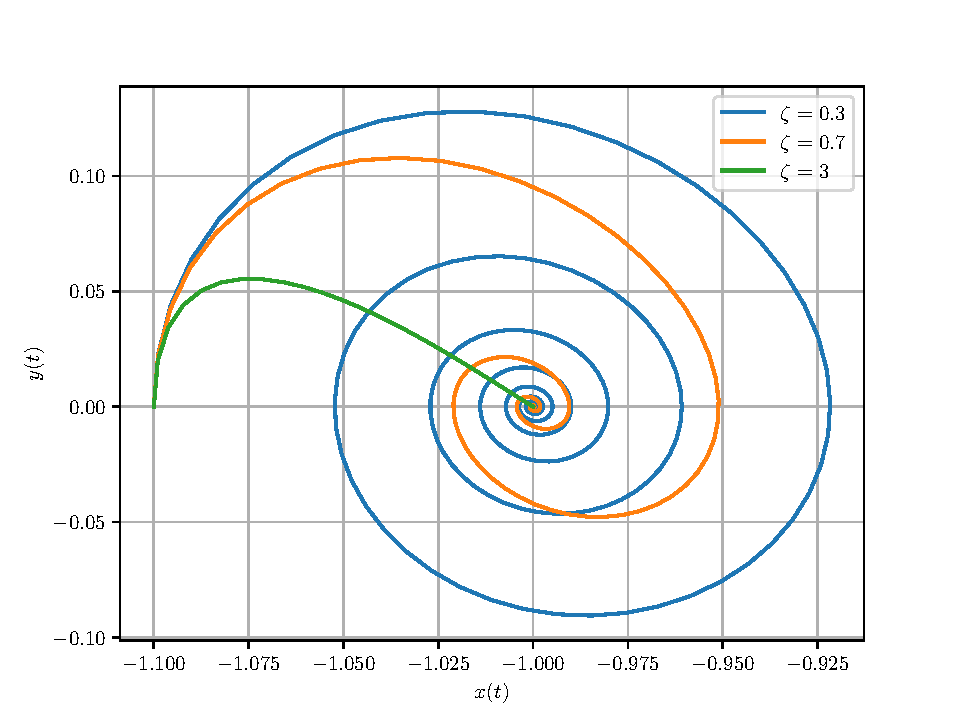
\includegraphics[width=1\textwidth]{figures/ex2_attractors.pdf}
        \caption{\gr{Περιοχές έλξης για διάφορα \( \zeta \).}}
        \label{fig:ex2_attractors}
    \end{figure}

    Παρακάτω παρουσιάζονται τα πορτρέτα κίνησης για μικρή απόσβεση,
    \( \zeta = 0.3 \) και μεγάλη \( \zeta = 0.7 \), και το πορτρέτο κίνησης
    για τις δύο τιμές του \( \zeta \).
    \begin{figure}[h]
        \centering
        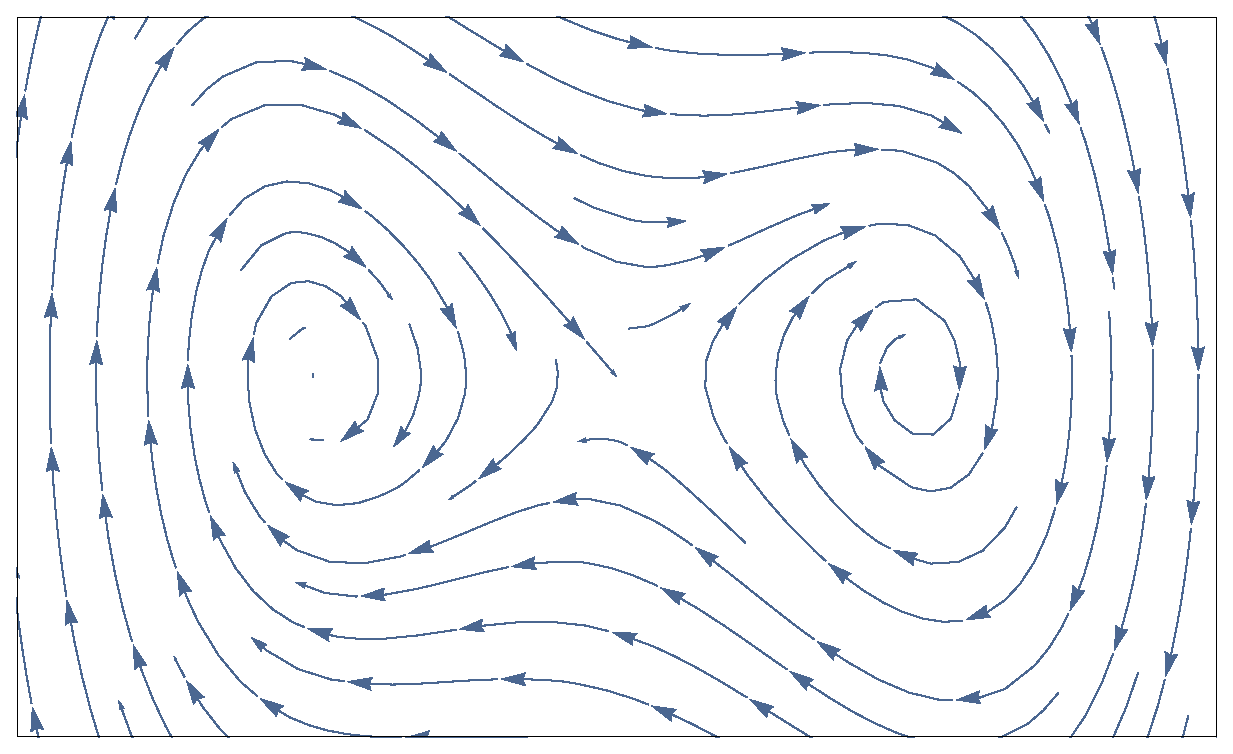
\includegraphics[width=0.8\textwidth]{figures/ex2_dampedDuffing03Vec.eps}
        \caption{\gr{Πορτρέτο κίνησης ταλαντωτή \tl{Duffing} με απόσβεση,
        \(\zeta = 0.3\).}}
        \label{fig:ex2_dampedDuffing03Vec}
    \end{figure}
    Στο σχήμα~\ref{fig:ex2_dampedDuffing0307Vec}, με το μπλε χρώμα είναι το πεδίο
    για \( \zeta = 0.3 \) και με το καφέ χρώμα το πεδίο για
    \( \zeta = 0.7 \). Από το σχήμα αυτό, αλλά και από το
    σχήμα~\ref{fig:ex2_attractors} είναι φανερό, ότι για μικρό \( \zeta \)
    έχουμε μεγαλύτερες ταλαντώσεις, όπως ήταν αναμενόμενο. Επίσης, από τα διαγράμματα
    αυτά και μόνο είναι φανερό ότι η μεγάλη απόσβεση μας πηγαίνει στα σημεία ισορροπίας
    ταχύτερα. Για μεγαλύτερη έμφαση παρουσιάζεται στο
    σχήμα~\ref{fig:ex2_dampedDuffing} η χρονική απόκριση των μεταβλητών για
    αποσβέσεις \( \zeta = 0.3 \) και \( \zeta = 0.7 \) αλλά και επίσης για
    απόσβεση \( \zeta = 2\sqrt{2} \) έτσι ώστε να φανεί η διαφορετική μορφή σύγκλισης.
    \begin{figure}[h!]
        \centering
        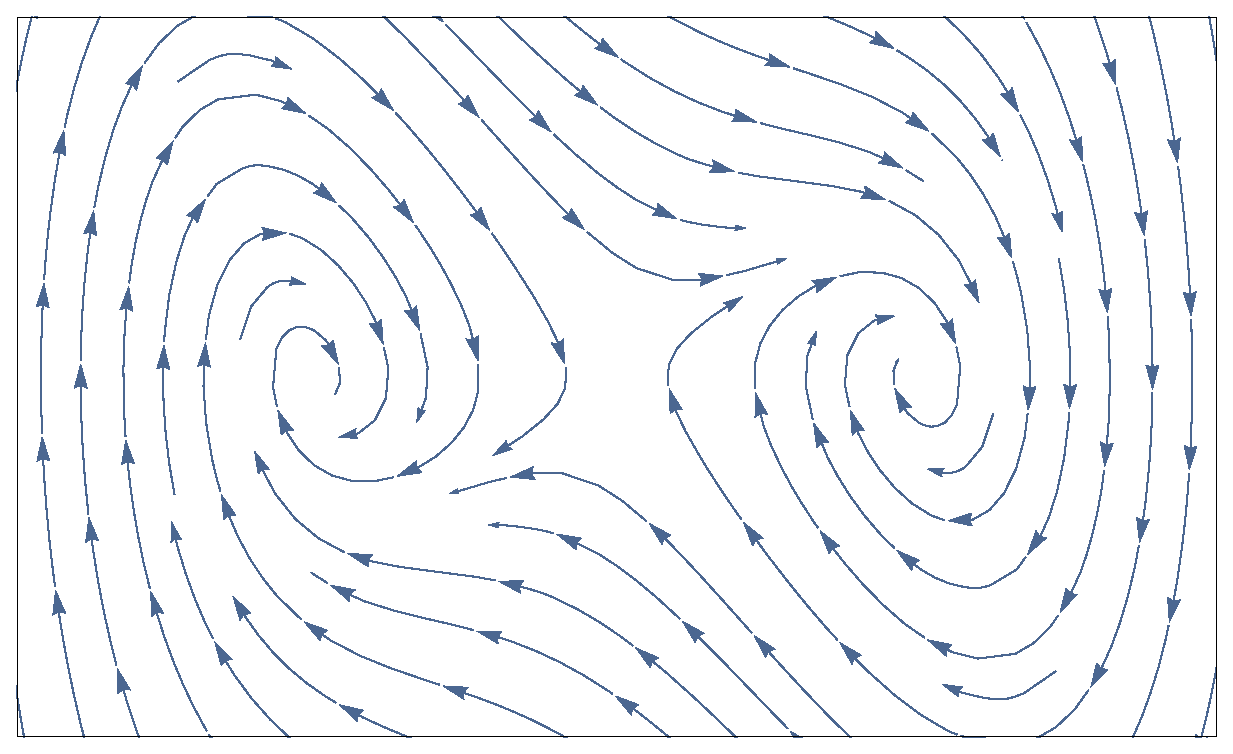
\includegraphics[width=0.8\textwidth]{figures/ex2_dampedDuffing07Vec.eps}
        \caption{\gr{Πορτρέτο κίνησης ταλαντωτή \tl{Duffing} με απόσβεση,
        \(\zeta = 0.7\).}}
        \label{fig:ex2_dampedDuffing07Vec}
    \end{figure}
    \begin{figure}[h!]
        \centering
        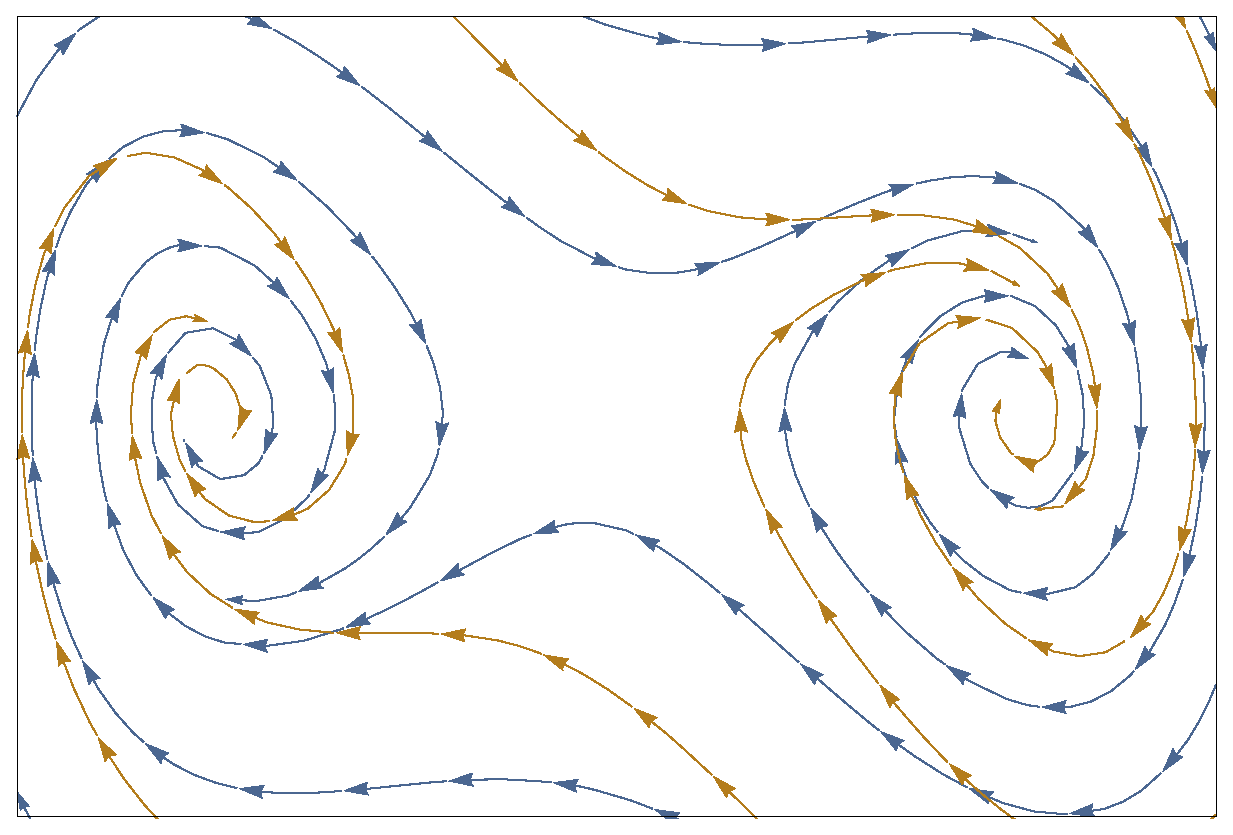
\includegraphics[width=0.8\textwidth]{figures/ex2_dampedDuffing0307Vec.eps}
        \caption{\gr{Πορτρέτο κίνησης ταλαντωτή \tl{Duffing}
                για \( \zeta = 0.3 \) (μπλε χρώμα) και για \( \zeta = 0.7 \) (καφέ
        χρώμα).}}
        \label{fig:ex2_dampedDuffing0307Vec}
    \end{figure}
    \begin{figure}[h!]
        \centering
        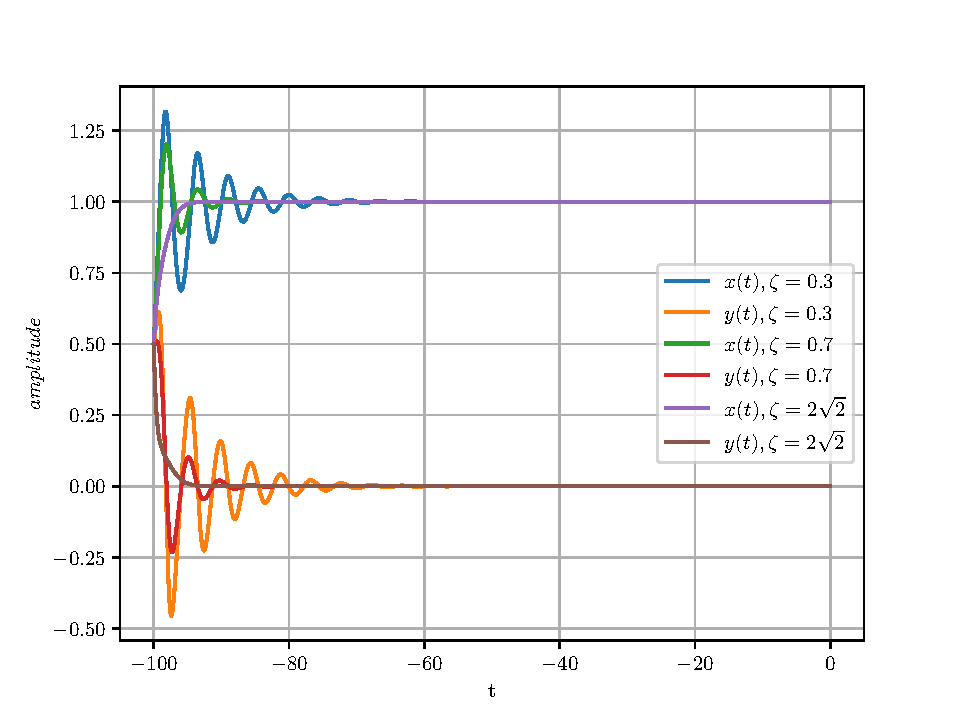
\includegraphics[width=1\textwidth]{figures/ex2_dampedDuffing.pdf}
        \caption{\gr{Απόκριση ταλαντωτή \tl{Duffing} για διάφορα \( \zeta \).}}
        \label{fig:ex2_dampedDuffing}
    \end{figure}
\end{solution}

\begin{exercise}{2016/17 3}
    \emph{Οι εξισώσεις \tl{Lorenz}}: Όπως είναι γνωστό το παρακάτω απλό σύστημα
    σε τρεις διαστάσεις που μελετήθηκε το \( 1963 \) από τον \tl{E. Lorenz}
    παρουσιάζει \enquote*{χαοτική συμπεριφορά} για κάποιες τιμές των παραμέτρων
    του.
    \begin{align*}
        \dot{x} &= \sigma(y - x) \\
        \dot{y} &= \rho x - y - xz \\
        \dot{z} &= \beta z + xy, \quad ( \sigma, \rho, beta > 0).
    \end{align*}
    Προς το παρόν, θα δούμε κάποια βασικά χαρακτηριστικά του.
    \begin{enumerate}[label= (\alph*)]
        \item Βρείτε τα σημεία ισορροπίας του και την εξάρτησή τους από τις
            παραμέτρους.
        \item Δείξτε ότι ο κάθετος άξονας \( z \) είναι αναλλοίωτη ευθεία για το
            σύστημα και περιγράψτε τη δυναμική πάνω του. Επίσης, δείξτε ότι το
            σύστημα έχει τη συμμετρία \( (x, y, z) \to (-x, -y, z) \).
        \item Δείξτε ότι
            \begin{enumerate}[label= (\roman*)]
                \item για \( 0 < \rho < 1 \), το σημείο ισορροπίας στο \( 0 \)
                    είναι ολικά ασυμπτωτικά ευσταθές, κάνοντας χρήση της
                    συνάρτησης \tl{Lyapunov}
                    \begin{equation*}
                        V(x, y, z) = \rho x^2 + \sigma(y^2 + z^2).
                    \end{equation*}
                \item για \( \rho > 1 \), το σημείο ισορροπίας \( 0 \) έχει
                    μονοδιάστατη ασταθή πολλαπλότητα \( W^u(0) \).
            \end{enumerate}
    \end{enumerate}
\end{exercise}
\begin{solution}{2016/17 3}
    (α). Τα σημεία ισορροπίας υπολογίζονται από τις σχέσεις
    \begin{align*}
        0 &= \sigma(y - x) \\
        0 &= \rho x - y - xz \\
        0 &= \beta z + xy
    \end{align*}
    Από την πρώτη σχέση προκύπτει
    \[
        y = x.
    \]
    Με αντικατάσταση αυτής στην τρίτη
    και λύνοντας ως προς \( z \) προκύπτει
    \[
        z = \frac{x^2}{\beta}.
    \]
    Τέλος, με αντικατάσταση των δύο παραπάνω σχέσεων στην δεύτερη έχουμε
    \[
        0 = \rho x - x \frac{x^2}{\beta} = x \left( \rho -1 - \frac{x^2}{\beta}
        \right),
    \]
    που σημαίνει \( x = 0 \), ή
    \begin{align*}
        0 &= \rho -1 - \frac{x^2}{\beta} \\
        x^2 &= \beta(\rho - 1),
    \end{align*}
    και για \( \rho > 1 \) προκύπτει \( x = \pm\sqrt{\beta(\rho - 1)} \).

    Τελικά, τα σημεία ισορροπίας είναι το \( \left(0, 0, 0\right) \) και αν \( \rho > 1 \) έχουμε
    και τα σημεία \( \left(\sqrt{\beta(\rho - 1)}, \sqrt{\beta(\rho - 1)}, \rho
    -1\right) \) και \( \left( -\sqrt{\beta(\rho - 1)}, -\sqrt{\beta(\rho - 1)},
    \rho -1 \right) \).

    Για να διαπιστώσουμε τη μορφή των σημείων ισορροπίας θα πάρουμε τη
    γραμμικοποίηση του συστήματος. Αν γράψουμε το σύστημα στη μορφή
    \begin{equation*}
        \begin{pmatrix}
            \dot{x} \\
            \dot{y} \\
            \dot{z}
        \end{pmatrix} = F(x, y, z) =
        \begin{pmatrix}
            \sigma(y - x) \\
            \rho x - y - xz \\
            \beta z + xy
        \end{pmatrix},
    \end{equation*}
    τότε η Ιακωβιανή είναι
    \begin{equation*}
        DF(x, y, z) =
        \begin{pmatrix}
            -\sigma & \sigma & 0 \\
            \rho - z & -1 & -x \\
            y & x & -\beta \\
        \end{pmatrix}.
    \end{equation*}
    Έτσι για την αρχή ισχύει
    \begin{equation*}
        DF(0, 0, 0) =
        \begin{pmatrix}
            -\sigma & \sigma & 0 \\
            \rho & -1 & 0 \\
            0 & 0 & -\beta \\
        \end{pmatrix}.
    \end{equation*}
    Είναι εμφανές ότι μία ιδιοτιμή είναι \( \lambda_1 = -\beta < 0\). Για να
    βρούμε τις άλλες δύο θα πάρουμε την ορίζουσα
    \begin{equation*}
        \det
        \begin{pmatrix}
            -\sigma - \lambda & \sigma \\
            \rho & -1 - \lambda \\
        \end{pmatrix}=
        (-\sigma - \lambda)(-1 - \lambda) - \sigma \rho,
    \end{equation*}
    που τελικά δίνει
    \begin{equation*}
        \lambda^2 + \lambda(\sigma + 1) + \sigma(1 - \rho) = 0.
    \end{equation*}
    Η διακρίνουσα της παραπάνω είναι
    \begin{equation*}
        \Delta = {(\sigma + 1)}^2 - 4\sigma(1 - \rho),
    \end{equation*}
    και οι ιδιοτιμές είναι
    \begin{equation*}
        \lambda_{2,3} = \frac{-(\sigma + 1) \pm \sqrt{\Delta}}{2}.
    \end{equation*}
    Αν \( \lambda_2 \) είναι η ιδιοτιμή που προκύπτει από το θετικό
    πρόσημο που είναι μπροστά από την τετραγωνική ρίζα και αντίστοιχα
    \( \lambda_3 \) η άλλη ιδιοτιμή, τότε προφανώς  \( \lambda_3 < 0 \). Θα
    δούμε, για την ιδιοτιμή \( \lambda_2 \). Οι ρίζες της είναι
    \begin{equation*}
        -(\sigma + 1) + \sqrt{{(\sigma + 1)}^2 - 4\sigma(1 - \rho)} = 0,
    \end{equation*}
    όπου υψώνοντας στο τετράγωνο προκύπτει
    \begin{equation*}
        {(\sigma + 1)}^2 - 4\sigma(1 - \rho) = {(\sigma + 1)}^2,
    \end{equation*}
    ή
    \begin{equation*}
        - 4\sigma(1 - \rho) = 0,
    \end{equation*}
    και επειδή \( \sigma > 0 \), προκύπτει \( \rho = 1 \).

    Άρα \( \lambda_2 < 0 \), όταν \( 0 < \rho < 1 \) και τότε, διότι
    \( \lambda_1, \lambda_3 < 0 \), από το θεώρημα
    \tl{Hartman-Grobman} το \( (0, 0, 0) \) είναι ασυμπτωτικά ευσταθές.

    Όταν \( \rho > 1 \), τότε \( \lambda_2 > 0 \) και επειδή
    \( \lambda_1, \lambda_3 < 0 \), η αρχή από το θεώρημα
    \tl{Hartman-Grobman} είναι σάγμα. Αυτό αποδεικνύει το ερώτημα (γ)
    \tl{ii}.

    Όταν \( \rho = 1 \), τότε \( \lambda_2 = 0 \) και \( \lambda_3 = -(\sigma +
    1) \) αλλά επειδή έχουμε μη υπερβολικό σημείο ισορροπίας δεν μπορούμε να
    χρησιμοποιήσουμε το θεώρημα \tl{Hartman-Grobman}. Η αντίστοιχη ανάλυση για
    τα άλλα δύο σημεία ισορροπίας είναι ιδιαίτερα πολύπλοκη και θα παραλειφθεί.

    (β). Το σύστημα έχει τη συμμετρία \( (x, y, z) \to (-x, -y, z) \) και
    φαίνεται εύκολα αν εφαρμόσουμε το μετασχηματισμό. Έτσι
    \begin{align*}
        -\dot{x} &= \sigma(-y + x) \\
        -\dot{y} &= -\rho x + y + xz \\
        \dot{z} &= -\beta z + (-x)(-y),
    \end{align*}
    όπου όμως το παραπάνω ισούται με το αρχικό
    \begin{align*}
        \dot{x} &= \sigma(y - x) \\
        \dot{y} &= \rho x - y - xz \\
        \dot{z} &= -\beta z + xy,
    \end{align*}
    και αυτό επιβεβαιώνει τη συμμετρία ως προς τον άξονα \( z \).

    Ένα σύνολο \( K \subset \mathbb{R}^n \) είναι αναλλοίωτο για τη ροή ενός
    διανυσματικού πεδίου εάν \( x \in K \Rightarrow \phi(x, t) \in K \).
    Επομένως, για να ένα σημείο \( z \in (0, 0, z) \) έχουμε
    \begin{align*}
        \dot{x} &= 0 \\
        \dot{y} &= 0 \\
        \dot{z} &= -\beta z,
    \end{align*}
    και άρα η ροή του διανυσματικού πεδίου, για οποιοδήποτε σημείο πάνω στον
    άξονα \( z \), παραμένει στον άξονα \( z \) για κάθε \( t \) και άρα είναι
    αναλλοίωτη ευθεία για το σύστημα.

    (γ) \tl{i}. Θα χρησιμοποιήσουμε τη συνάρτηση \tl{Lyapunov}
    \begin{equation*}
        V(x, y, z) = \rho x^2 + \sigma(y^2 + z^2),
    \end{equation*}
    για \( 0 < \rho < 1 \) και για το σημείο \( (0, 0, 0) \). Αρχικά στο σημείο
    αυτό προφανώς ισχύει \( V(0, 0, 0) = 0 \) και για \( (x, y, z) \neq (0, 0,
    0) \) βλέπουμε ότι \( V(x, y, z) > 0 \). Στη συνέχεια θα υπολογίσουμε το
    ρυθμό μεταβολής της συνάρτησης \tl{Lyapunov}. Έτσι έχουμε
    \begin{align*}
        \frac{d}{dt}V(x(t), y(t), z(t))
        &= 2\rho x \dot{x} + 2\sigma y \dot{y} + 2 \sigma z \dot{z} \\
        &= 2\rho x (\sigma(y - x)) + 2\sigma y (\rho x - y - xz) + 2 \sigma z
        (-\beta z + xy) \\
        &= 2\rho x\sigma y - 2\rho\sigma x^2 + 2\sigma y\rho x - 2\sigma y^2 -
        2\sigma yxz - 2 \sigma\beta z^2 + 2\sigma zxy \\
        &= -2\sigma \left( -2\rho xy + \rho x^2 + y^2 + \beta z^2 \right) \\
        &= -2\sigma \left( -2\rho xy + \rho x^2 + y^2 + \beta z^2 + \rho^2 x^2 -
        \rho^2x^2\right) \\
        &= -2\sigma \left[ {(\rho x - y)}^2 + \beta z^2 + \rho x^2(1 -
        \rho)\right].
    \end{align*}
    Δεδομένου ότι \( 0 < \rho < 1 \), ισχύει \( \dot{V} < 0 \) καθώς όλοι οι
    όροι είναι τετραγωνικοί. Έτσι για κάθε \( (x, y, z) \neq (0, 0, 0) \) και
    συνεπώς είναι ολικά ασυμπτωτικά ευσταθές σημείο ισορροπίας.
\end{solution}

\begin{exercise}{2016/17 4}
    \emph{Το απλό εκκρεμές} είναι το σύστημα, σε κανονική μορφή,
    \begin{align*}
        \dot{x} &= y \\
        \dot{y} &= -a y - \sin{x}
    \end{align*}
    και περιγράφει ένα απλό εκκρεμές, αλλά και τη δυναμική ενός περιστρεφόμενου
    σώματος γύρω από έναν άξονα.

    Για μηδενική απόσβεση \( a = 0 \) το σύστημα είναι Χαμιλτονιανό. Για θετική
    απόσβεση \( a > 0 \), τα σημεία ισορροπίας δεν μετακινούνται, αλλά αλλάζει η
    ευστάθειά τους.

    \begin{enumerate}[label= (\alph*)]
        \item Δώστε τυπικά πορτρέτα κίνησης για διάφορες θετικές τιμές του
            \( a \) και περιγράψτε τις ποιοτικές αλλαγές στη δυναμική
            συμπεριφορά που παρατηρούνται.
        \item Εφαρμόζεται τώρα μία σταθερή ροπή \( T \) στο σύστημα, ώστε το
            σύστημα είναι
            \begin{align*}
                \dot{x} &= y \\
                \dot{y} &= -a y - \sin{x} + T.
            \end{align*}
            Τα σημεία ισορροπίας μετακινούνται.
            \begin{enumerate}[label= (\roman*)]
                \item Θεωρούμαι πρώτα την περίπτωση \( 0 < T < 1 \). Με κατάλληλη
                    αναφορά στο αντίστοιχο Χαμιλτονιανό σύστημα (δηλαδή για
                    \( a = 0 \), για το οποίο και κάνετε το πορτρέτο
                    κίνησης), δείξτε πως η περιοχή έλξης παραμένει μεν σταθερή, αλλά
                    είμαστε πολύ κοντά σε αστάθεια, καθώς το ευσταθές σημείο
                    πλησιάζει το σάγμα και χρειάζεται μικρή ενέργεια για να βγούμε
                    (και τι γίνεται μετά;).
                \item Δείξτε ότι για \( T > 1 \) δεν υπάρχουν σημεία ισορροπίας.
                    Το σύστημα παρ᾽ όλα αυτά παραμένει ευσταθές λόγω των
                    αποσβέσεων. Δώστε το πορτρέτο κίνησης και δείξτε ότι υπάρχει
                    ευσταθής οριακός κύκλος στον κύλινδρο (αυστηρή απόδειξη
                    γίνεται με χρήση του θεωρήματος των \tl{Poincar\'{e}-Bendixson}).
            \end{enumerate}
    \end{enumerate}
\end{exercise}
\begin{solution}{2016/17 4}
    (α). Τα σημεία ισορροπίας του απλού εκκρεμούς υπολογίζονται από
    \begin{align*}
        0 &= y \\
        0 &= -a y - \sin{x},
    \end{align*}
    που σημαίνει ότι \( x = k\pi \) με \( k \in \mathbb{Z} \). Αν γράψουμε τις
    σχέσεις στη μορφή
    \[
        \begin{pmatrix}
            \dot{x} \\
            \dot{y}
        \end{pmatrix} = F(x, y) =
        \begin{pmatrix}
            y \\
            -a y - \sin{x}
        \end{pmatrix},
    \]
    και πάρουμε τη γραμμικοποίηση προκύπτει
    \[
        DF(x, y) =
        \begin{pmatrix}
            0 & 1 \\
            -\cos{x} & -a
        \end{pmatrix}.
    \]
    Στο \( (0, 0) \) ή γενικότερα στο \( (2k\pi, 0) \) ισχύει
    \[
        DF(2k\pi, 0) =
        \begin{pmatrix}
            0 & 1 \\
            -1 & -a
        \end{pmatrix},
    \]
    και οι ιδιοτιμές της είναι
    \[
        \det
        \begin{pmatrix}
            -\lambda & 1 \\
            -1 & -a - \lambda
        \end{pmatrix}
        = \lambda^2 + \lambda a + 1.
    \]
    Η παραπάνω έχει διακρίνουσα
    \[
        \Delta = a^2 - 4.
    \]
    Όταν \( \Delta < 0 \), δηλαδή όταν \( 0 < a < \sqrt{2} \) τότε οι ρίζες
    \[
        \lambda = \frac{-a \pm i \sqrt{a^2 - 4}}{2},
    \]
    είναι μιγαδικές με αρνητικό πραγματικό μέρος και συνεπώς από το θεώρημα
    \tl{Hartman-Grobman} το σημείο είναι ασυμπτωτικά ευσταθές για το μη-γραμμικό
    σύστημα, για \( a > 0 \) και έχει τη μορφή ευσταθούς εστίας. Όταν \( a = 0 \)
    δε μπορούμε να εφαρμόσουμε το θεώρημα, αλλά γνωρίζουμε ότι έχει συμπεριφορά
    κέντρου από τη μελέτη του Χαμιλτονιανού συστήματος καθώς στο \( 2k\pi \) η
    συνάρτηση δυναμικού παρουσιάζει ελάχιστο.

    Αν \( \Delta > 0 \) τότε εύκολα φαίνεται ότι
    \[
        \lambda_1 = \frac{-a + \sqrt{a^2 - 4}}{2} < 0, \quad
        \lambda_2 = \frac{-a - \sqrt{a^2 - 4}}{2} < 0.
    \]
    Συνεπώς από το θεώρημα \tl{Hartman-Grobman} το σημείο είναι
    ασυμπτωτικά ευσταθές για το μη-γραμμικό σύστημα, με μορφή ευσταθούς κόμβου.
    Αυτή η περίπτωση φυσικά εμφανίζεται μόνο όταν \( a > 0 \).

    Τέλος, για \( \Delta = 0 \) τότε \( a = \sqrt{2} \) και προκύπτει η διπλή
    ιδιοτιμή \( \lambda_{1,2} = \frac{-a}{2} \), που είναι φυσικά ασυμπτωτικά
    ευσταθής.

    Αντίστοιχα για τα σημεία ισορροπίας \( ((2k + 1)\pi, 0) \) από την γραμμικοποίηση προκύπτει
    \[
        DF((2k + 1)\pi, 0) = \begin{pmatrix}
            0 & 1 \\
            -1 & -a
        \end{pmatrix},
    \]
    και οι ιδιοτιμές της είναι
    \[
        \det
        \begin{pmatrix}
            -\lambda & 1 \\
            1 & -a - \lambda
        \end{pmatrix}
        = \lambda^2 + \lambda a - 1.
    \]
    Η παραπάνω έχει διακρίνουσα
    \[
        \Delta = a^2 + 4 > 0,
    \]
    και οι ιδιοτιμές είναι
    \[
        \lambda_1 = \frac{-a + \sqrt{a^2 + 4}}{2} > 0, \quad
        \lambda_2 = \frac{-a - \sqrt{a^2 + 4}}{2} < 0.
    \]
    Συνεπώς από το θεώρημα \tl{Hartman-Grobman} το σημείο είναι
    σάγμα για το μη-γραμμικό σύστημα.

    Στο σχήμα~\ref{fig:ex4_undampedPendComb} απεικονίζεται το πορτρέτο κίνησης
    του απλού εκκρεμούς, χωρίς απόσβεση και χωρίς κάποια εξωτερική ροπή.
    \begin{figure}[h]
        \centering
        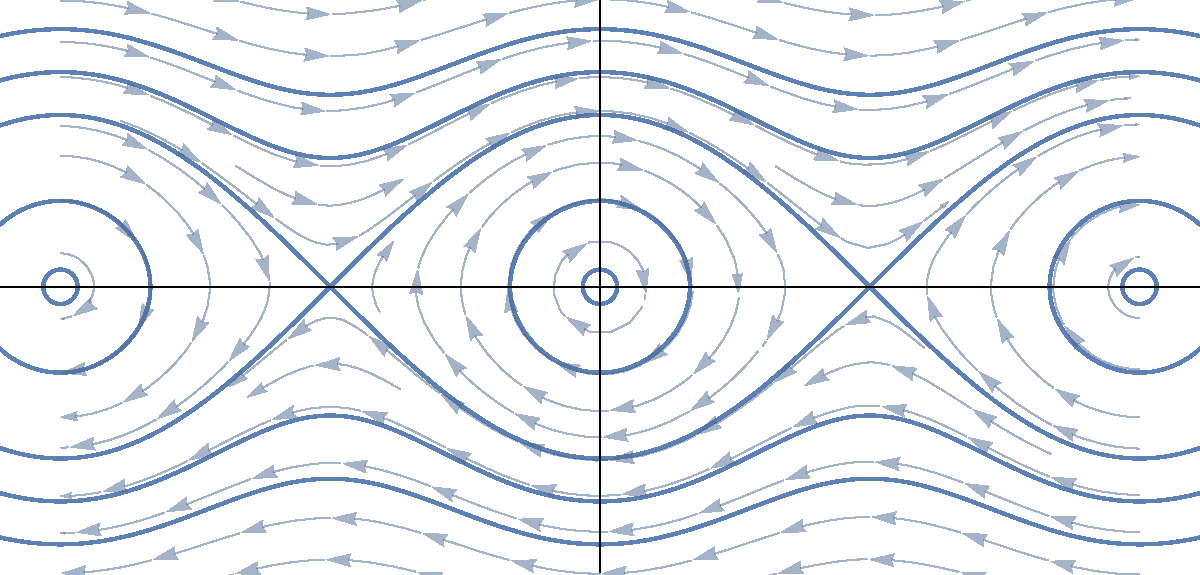
\includegraphics[width=0.8\textwidth]{figures/ex4_undampedPendComb.pdf}
        \caption{\gr{Πορτρέτο κίνησης εκκρεμούς, \( a = 0, T = 0 \)}}
        \label{fig:ex4_undampedPendComb}
    \end{figure}
    Το σύστημα στην περίπτωση αυτό είναι Χαμιλτονιανό με συνολική ενέργεια
    \[
        H(x, y) = \frac{1}{2}y^2 + U(x),\quad U(x) = - \cos{x},
    \]
    και οι ισοϋψείς καμπύλες του σχήματος είναι
    \[
        y = \pm \sqrt{2(h_0 + \cos{x})}.
    \]
    Κοιτώντας το διάστημα \( (-\pi, \pi) \), βλέπουμε ότι στο \( (0, 0) \) έχουμε
    συμπεριφορά κέντρου και σημεία κοντά σε αυτό έχουν αυτή τη συμπεριφορά. Σημεία
    που βρίσκονται πάνω στις τροχιές των σαγμάτων ή πάνω από αυτές θα παραμείνουν
    για πάντα ασταθή και ποτέ δεν θα ισορροπήσουν. Επομένως, αυτό το
    \enquote*{μάτι} είναι η διαχωριστική καμπύλη (\tl{separatrix}). Τέλος, η
    τροχιά που τείνει στο \( \pi \) ή στο \( -\pi \) προέρχεται από την ευσταθή
    ιδιοτιμή και ουσιαστικά αντιπροσωπεύει την κάθετη θέση που δύναται να
    ισορροπήσει το εκκρεμές.

    Στο σχήμα~\ref{fig:ex4_damped05Comb}, απεικονίζεται το πορτρέτο κίνησης
    του απλού εκκρεμούς, με απόσβεση \( a = 0.5 \) και χωρίς κάποια εξωτερική ροπή.
    \begin{figure}[h]
        \centering
        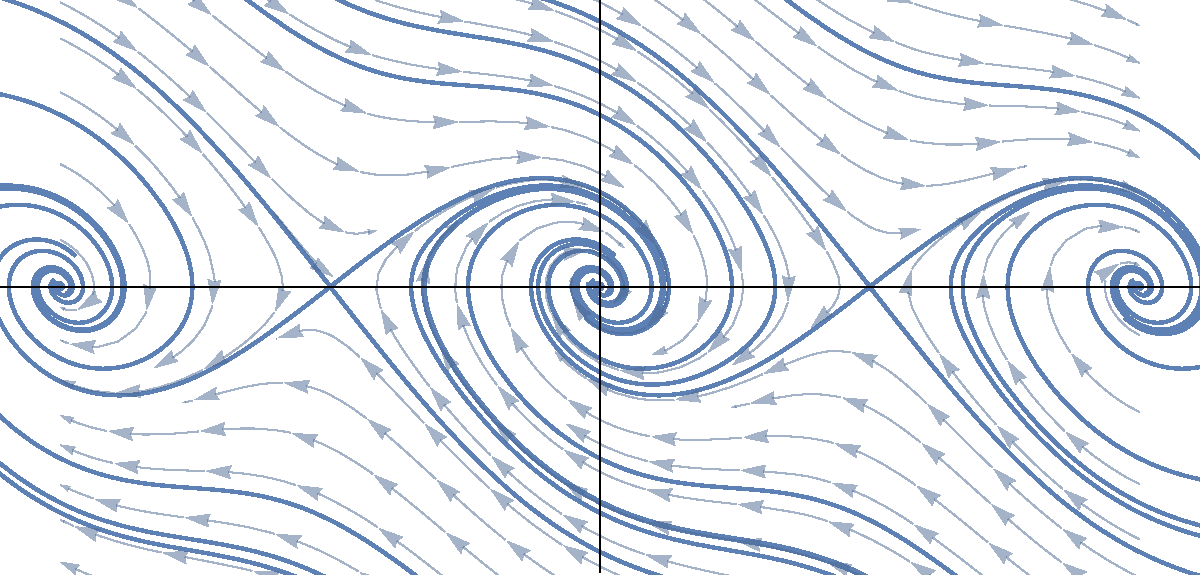
\includegraphics[width=0.8\textwidth]{figures/ex4_damped05Comb.pdf}
        \caption{\gr{Πορτρέτο κίνησης εκκρεμούς, \( a = 0.5, T = 0 \)}}
        \label{fig:ex4_damped05Comb}
    \end{figure}
    Όπως δείξαμε παραπάνω, και επικεντρώνοντας την προσοχή μας στο διάστημα
    \( (-\pi,\pi) \), η προσθήκη απόσβεσης μετατρέπει το σημείο \( (0, 0) \) από
    κέντρο σε ασυμπτωτικά ευσταθές σημείο ισορροπίας. Μία επιπλέον σημαντική αλλαγή
    που επιφέρει η απόσβεση είναι ότι αλλάζει (μεγαλώνει) την περιοχή έλξης. Όπως
    φαίνεται στο σχήμα~\ref{fig:ex4_damped05Comb}, οι τροχιές που τείνουν στο
    \( -\pi \) και \( \pi \) αντίστοιχα, είναι οι διαχωριστικές καμπύλες και
    είναι επίσης οι καμπύλες που αντιστοιχούν στην κάθετη θέση του εκκρεμούς.
    Η περιοχή έλξης για το σημείο ισορροπίας \( (0, 0) \) είναι αριστερά και
    δεξιά των διαχωριστικών καμπυλών του \( -\pi \) και \( \pi \) αντίστοιχα.

    Στο σχήμα~\ref{fig:ex4_damped1Comb}, απεικονίζεται το πορτρέτο κίνησης
    του απλού εκκρεμούς, με απόσβεση \( a = 1 \) και χωρίς κάποια εξωτερική ροπή.
    \begin{figure}[h]
        \centering
        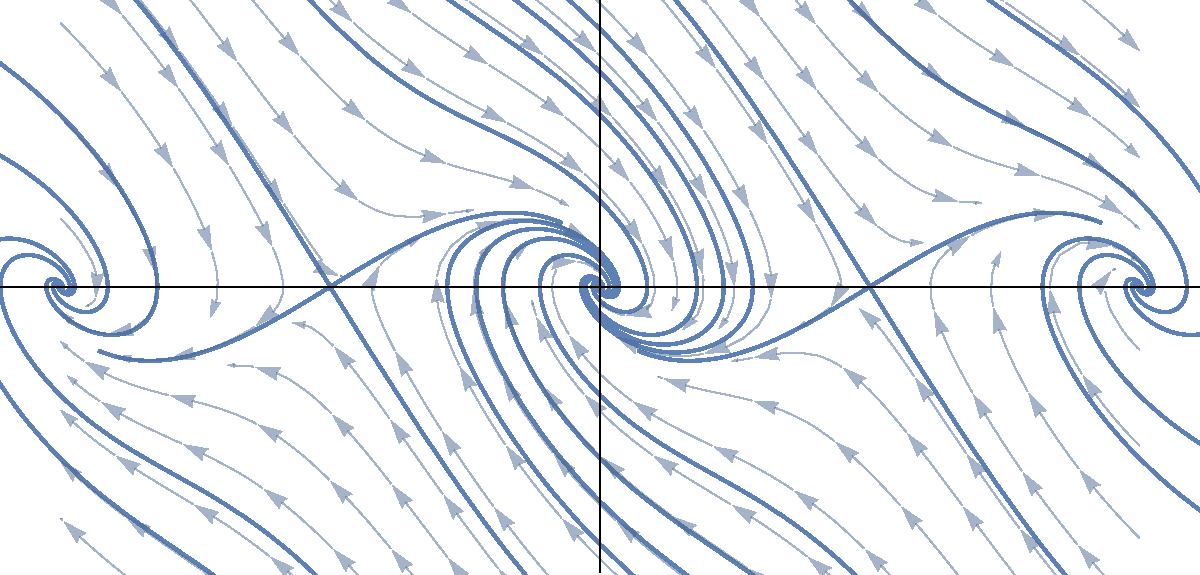
\includegraphics[width=0.8\textwidth]{figures/ex4_damped1Comb.pdf}
        \caption{\gr{Πορτρέτο κίνησης εκκρεμούς, \( a = 1, T = 0 \)}}
        \label{fig:ex4_damped1Comb}
    \end{figure}
    Δεν έχουμε κάποια ποιοτική αλλαγή σε σχέση με την περίπτωση όπου είχαμε
    \( a = 0.5 \). Δηλαδή ισχύει ότι και πριν. Η ουσιαστική διαφορά τους είναι
    ο ρυθμός σύγκλισης στο σημείο ισορροπίας. Με την αύξηση της απόσβεσης οι
    ταλαντώσεις μειώνονται αισθητά και αυτό αντικατοπτρίζεται στο
    σχήμα~\ref{fig:ex4_damped1Comb}.

    (β) \tl{i}. Περνάμε στην περίπτωση όπου εφαρμόζεται μία σταθερή ροπή
    \( T \) στο σύστημα, ώστε οι εξισώσεις να είναι
    \begin{align*}
        \dot{x} &= y \\
        \dot{y} &= -a y - \sin{x} + T,
    \end{align*}
    με \( 0 < T < 1 \). Υπολογίζοντας τα σημεία ισορροπίας προκύπτει
    \begin{align*}
        0 &= y \\
        0 &= -a y - \sin{x} + T,
    \end{align*}
    που συνεπάγεται
    \[
        \sin{x} = T.
    \]
    Η παραπάνω έχει τις λύσεις συναρτήσει τις ροπής
    \begin{align*}
        x_1(T) &= 2k\pi + \arcsin{T} \\
        x_2(T) &= (2k + 1)\pi - \arcsin{T},
    \end{align*}
    για \( k \in \mathbb{Z} \).
    \begin{figure}[h]
        \centering
        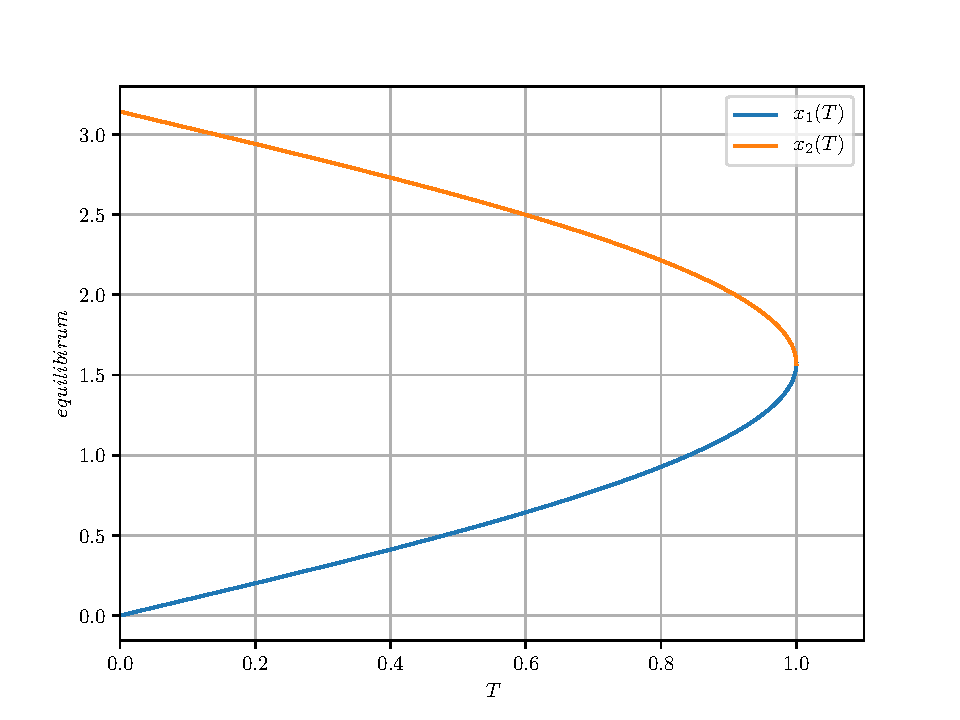
\includegraphics[width=0.9\textwidth]{figures/ex4_equilibriumPerTorque.pdf}
        \caption{\gr{Σημεία ισορροπίας συναρτήσει της ροπής \( T \) }}
        \label{fig:ex4_equilibriumPerTorque}
    \end{figure}
    Επικεντρώνουμε την προσοχή μας στο διάστημα \( (-\pi, \pi) \), δηλαδή για
    \( k = 0 \). Στο σχήμα~\ref{fig:ex4_equilibriumPerTorque} βλέπουμε την
    επιρροή που έχει η ροπή στα σημεία ισορροπίας. Καθώς αυξάνεται η ροπή τα
    δύο σημεία ισορροπίας \( x_1 \) και \( x_2 \) που αρχικά, για μηδενική
    ροπή ήταν στο \( (0, 0) \) και \( (\pi, 0) \) αντίστοιχα, πλησιάζουν μεταξύ τους
    μέχρι την οριακή τιμή της ροπής \( T = 1 \) όπου αυτά τα δύο σημεία
    ισορροπίας ταυτίζονται. Φυσικά όσο μεγαλώνει η ροπή, τόσο πλησιάζουν τα
    σημεία μεταξύ τους, που σημαίνει ότι όλο και πιο μικρές διαταραχές θα μας
    κάνουν το σύστημα ασταθές.
    \begin{figure}[h]
        \centering
        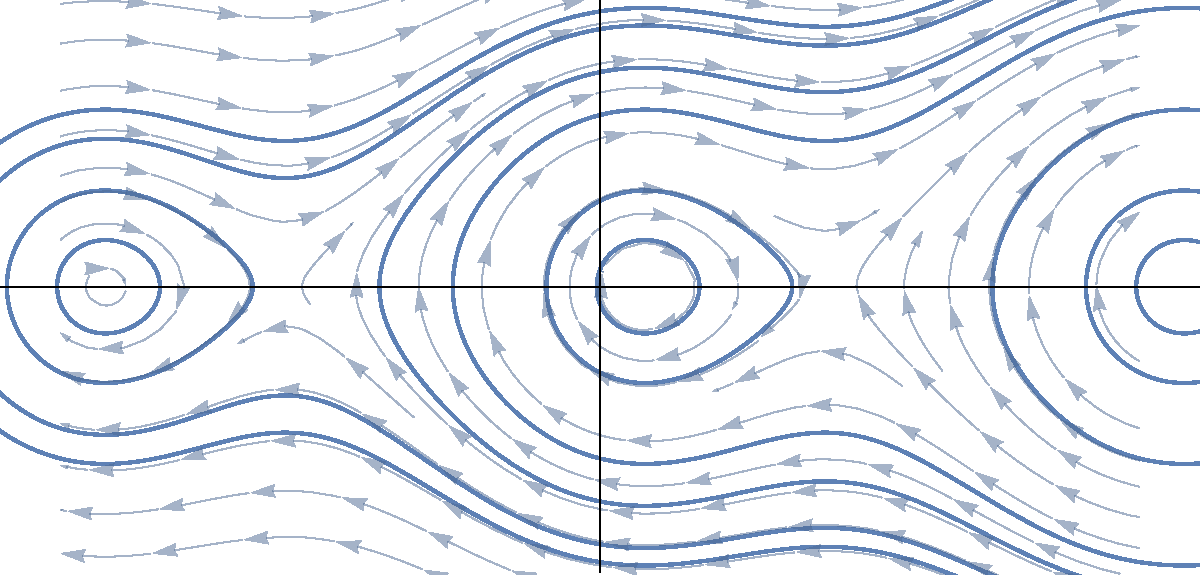
\includegraphics[width=0.8\textwidth]{figures/ex4_torque05Comb.pdf}
        \caption{\gr{Πορτρέτο κίνησης εκκρεμούς, \( a = 0, T = 0.5 \)}}
        \label{fig:ex4_torque05Comb}
    \end{figure}
    \begin{figure}[h]
        \centering
        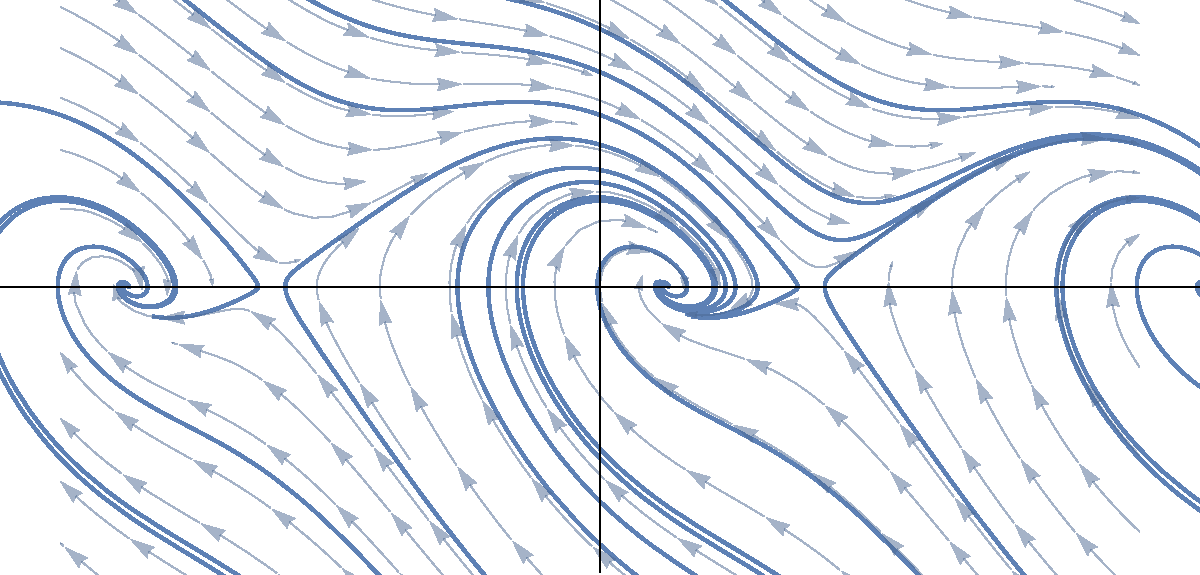
\includegraphics[width=0.8\textwidth]{figures/ex4_torque07damped07Comb.pdf}
        \caption{\gr{Πορτρέτο κίνησης εκκρεμούς, \( a = 0.7, T = 0.7 \)}}
        \label{fig:ex4_torque07damped07Comb}
    \end{figure}

    Στο σχήμα~\ref{fig:ex4_torque05Comb} βλέπουμε το πορτρέτο κίνησης για το
    εκκρεμές χωρίς απόσβεση και με ροπή \( T = 0.5 \). Παρατηρούμε ότι η ροπή
    μετακίνησε το σημείο ισορροπίας από το \( (0, 0) \) και το πήγε στο
    \( (0.52359, 0) \), ενώ το άλλο από το \( (\pi, 0) \) και το πήγε στο
    \( (2.6179, 0) \).

    Στο σχήμα~\ref{fig:ex4_torque05Comb} βλέπουμε το πορτρέτο κίνησης για το
    εκκρεμές με απόσβεση \( a = 0.7 \) και με ροπή \( T = 0.7 \). Παρατηρούμε
    ότι η ροπή μετακίνησε τα σημεία ισορροπίας ακόμα παραπάνω,
    από το \( (0, 0) \) στο \( (0.7753, 0) \), ενώ το άλλο από το \( (\pi, 0) \)
    στο \( (2.3661, 0) \). Όπως είναι φανερό από τα σχήματα, αλλά και από τις
    εξισώσεις, η ροπή δεν επηρεάζει τον τύπο των σημείων ισορροπίας.

    (β) \tl{ii}. Περνάμε στην περίπτωση όπου εφαρμόζεται μία σταθερή ροπή
    \( T > 1\) στο σύστημα, ώστε οι εξισώσεις να είναι
    \begin{align*}
        \dot{x} &= y \\
        \dot{y} &= -a y - \sin{x} + T.
    \end{align*}
    Υπολογίζοντας τα σημεία ισορροπίας προκύπτει
    \begin{align*}
        0 &= y \\
        0 &= -a y - \sin{x} + T,
    \end{align*}
    που συνεπάγεται
    \[
        \sin{x} = T.
    \]
    Η παραπάνω προφανώς για \( T > 1 \) δεν έχει λύσεις, και άρα το σύστημα δεν
    έχει σημεία ισορροπίας στην περίπτωση αυτή.
    \begin{figure}[h!]
        \centering
        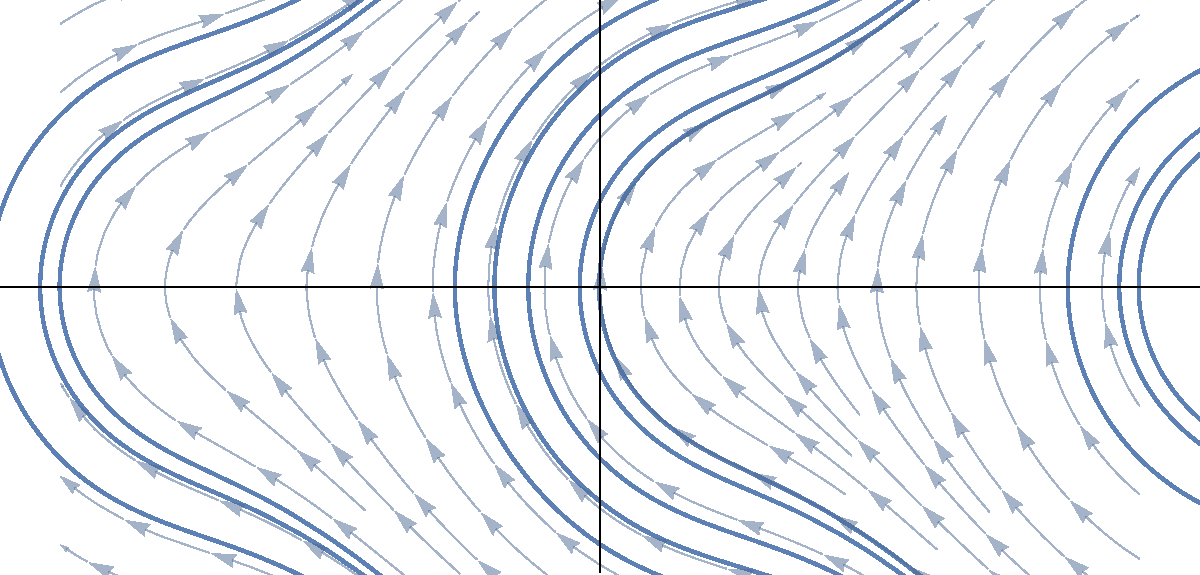
\includegraphics[width=0.8\textwidth]{figures/ex4_torque2Comb.pdf}
        \caption{\gr{Πορτρέτο κίνησης εκκρεμούς, \( a = 0, T = 2 \)}}
        \label{fig:ex4_torque2Comb}
    \end{figure}
    \begin{figure}[h!]
        \centering
        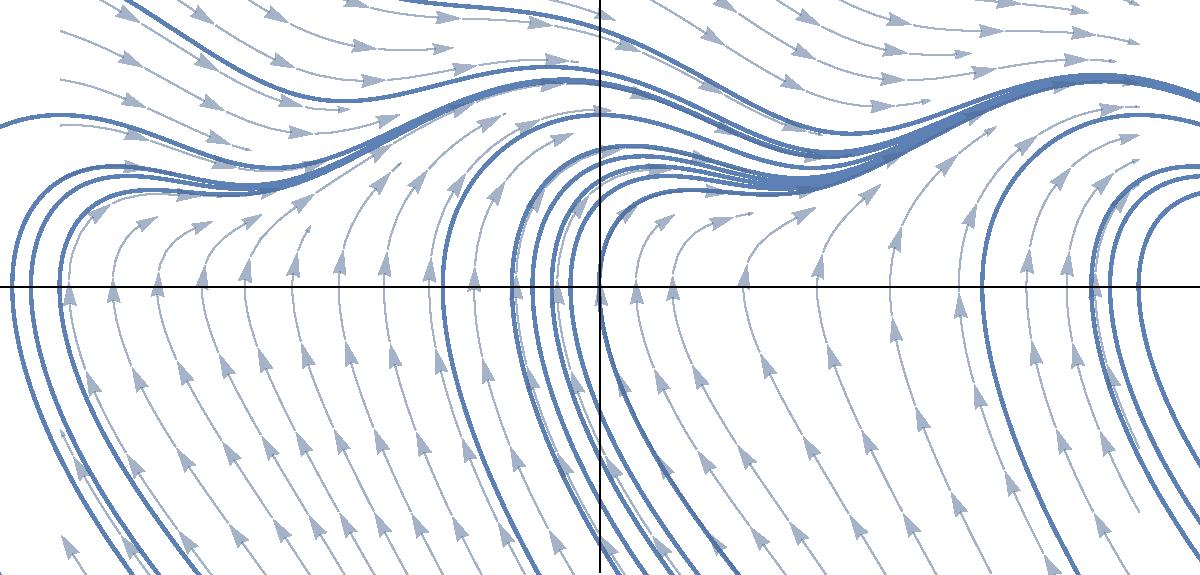
\includegraphics[width=0.8\textwidth]{figures/ex4_torque2damped1Comb.pdf}
        \caption{\gr{Πορτρέτο κίνησης εκκρεμούς, \( a = 1, T = 2 \)}}
        \label{fig:ex4_torque2damped1Comb}
    \end{figure}
    \begin{figure}[h!]
        \centering
        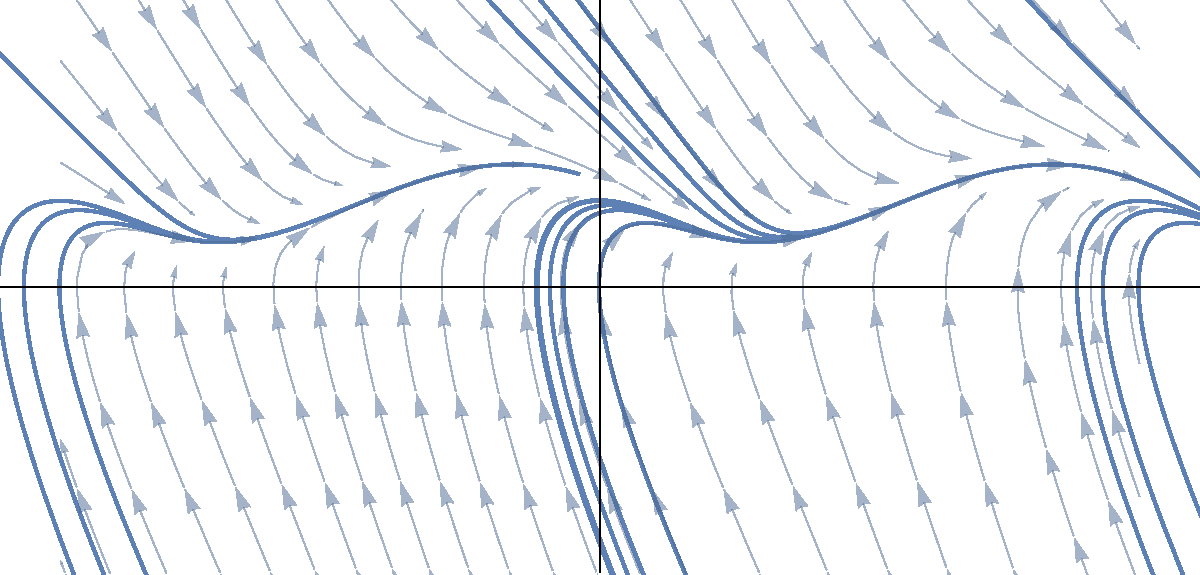
\includegraphics[width=0.8\textwidth]{figures/ex4_torque2damped2Comb.pdf}
        \caption{\gr{Πορτρέτο κίνησης εκκρεμούς, \( a = 2, T = 2 \)}}
        \label{fig:ex4_torque2damped2Comb}
    \end{figure}

    Στο σχήμα~\ref{fig:ex4_torque2Comb} βλέπουμε το πορτρέτο κίνησης για το
    εκκρεμές χωρίς απόσβεση και με ροπή \( T = 2 \). Παρατηρούμε ότι χωρίς
    απόσβεση το σύστημα είναι ασταθές.

    Στα σχήματα~\ref{fig:ex4_torque2damped1Comb}
    και~\ref{fig:ex4_torque2damped2Comb} βλέπουμε τα πορτρέτα κίνησης για το
    εκκρεμές με απόσβεση \( a = 1 \) και \( a = 2 \) αντίστοιχα και με ροπή
    \( T = 2 \). Παρατηρούμε ότι με την ύπαρξη της απόσβεσης και με την αύξηση
    αυτής, δημιουργείται ευσταθής οριακός κύκλος.
\end{solution}

\begin{exercise}{2016/17 5}
    \begin{enumerate}[label= (\alph*)]
        \item Μελετήστε το σύστημα στο επίπεδο
            \[
                \dot{x} = 2x - x^2, \quad \dot{y} = -y + xy.
            \]
            Βρείτε τα σημεία ισορροπίας, τον τύπο τους, καθώς και τις ευσταθείς
            και ασταθείς πολλαπλότητες καθενός από αυτά.

            Η \emph{θεωρία της δομικής ευστάθειας} λέει ότι, γενικά, κάθε ασταθής
            πολλαπλότητα ενός σημείου ισορροπίας (ή οριακού κύκλου) τέμνει την
            ευσταθή πολλαπλότητα άλλου σημείου ισορροπίας ή οριακού κύκλου
            \emph{εγκάρσια}.

            Δείξτε ότι στο παράδειγμα αυτό η τομή δεν είναι εγκάρσια. Είναι
            λοιπόν φυσικό να αναμένουμε ότι μικρές διαταραχές καταστρέφουν την
            μη-εγκάρσια αυτή τομή. Περιγράψτε τρόπους να γίνει αυτό.
            \emph{Υπόδειξη: επιλέξτε σημείο πάνω στην τροχιά που συνδέει τα
                σημεία ισορροπίας και με χρήση του κυτίου ροής (\tl{flow box})
            αλλάξτε τοπικά το διανυσματικό πεδίο}.
        \item Αναγνωρίστε παρόμοιες μη-εγκάρσιες τομές αναλλοίωτων πολλαπλοτήτων
            στις Χαμιλτονιανές περιπτώσεις των συστημάτων \tl{Duffing} και απλού
            εκκρεμούς.

            Συζητήστε κατά πόσο μπορούμε να φέρουμε τα συστήματα αυτά σε
            \enquote*{γενική θέση}, μένοντας όμως στην κατηγορία των
            Χαμιλτονιανών συστημάτων.
    \end{enumerate}
\end{exercise}
\begin{solution}{2016/17 5}
    (α). Τα σημεία ισορροπίας του συστήματος από την πρώτη σχέση είναι
    \begin{align*}
        0 &= 2x - x^2 \\
        0 &= x(2- x),
    \end{align*}
    άρα \( x = 0 \) ή \( x = 2 \). Από τη δεύτερη σχέση έχουμε
    \[
        0 = -y + xy.
    \]
    Άρα για \( x = 0 \) προκύπτει \( y = 0 \). Για \( x = 2 \) προκύπτει \( y =
    0 \). Ακόμα η δεύτερη εξίσωση μηδενίζεται για \( x = 1 \) και άρα εκεί το
    διανυσματικό πεδίο θα είναι παράλληλο το άξονα \( x \). Αν γράψουμε τις
    σχέσεις ως
    \[
        \begin{pmatrix}
            \dot{x} \\
            \dot{y}
        \end{pmatrix} = F(x, y)
        \begin{pmatrix}
            2x - x^2 \\
            -y + xy
            \dot{y}
        \end{pmatrix},
    \]
    τότε η γραμμικοποίηση είναι
    \[
        DF(x, y) =
        \begin{pmatrix}
            2 - 2x & 0 \\
            y & -1 + x
        \end{pmatrix}.
    \]
    Για το σημείο ισορροπίας στο \( (0, 0) \) έχουμε
    \[
        DF(0, 0) =
        \begin{pmatrix}
            2 & 0 \\
            0 & -1
        \end{pmatrix},
    \]
    άρα οι ιδιοτιμές είναι \( \lambda_1 = 2 \), που αντιπροσωπεύει την ασταθή πολλαπλότητα
    και \( \lambda_2 = -1 \), που αντιπροσωπεύει την ευσταθή πολλαπλότητα. Ο ευσταθής
    αναλλοίωτος υποχώρος \( E^s = \{ (x, y)\in \mathbb{R}^2: x = 0 \} \), και ο αντίστοιχος
    ασταθής αναλλοίωτος υποχώρος είναι \( E^u = \{ (x, y)\in \mathbb{R}^2: y = 0 \} \).
    Από το θεώρημα \tl{Hartman-Grobman} προκύπτει ότι το αρχικό μη-γραμμικό σύστημα είναι σάγμα
    στο \( (0, 0) \).

    Για το σημείο ισορροπίας στο \( (2, 0) \) έχουμε
    \[
        DF(0, 0) =
        \begin{pmatrix}
            -2 & 0 \\
            0 & 1
        \end{pmatrix},
    \]
    άρα οι ιδιοτιμές είναι \( \lambda_1 = 1 \), που αντιπροσωπεύει την ασταθή πολλαπλότητα
    και \( \lambda_2 = -2 \), που αντιπροσωπεύει την ευσταθή πολλαπλότητα. Ο ευσταθής
    αναλλοίωτος υποχώρος \( E^s = \{ (x, y)\in \mathbb{R}^2: y = 0 \} \), και ο αντίστοιχος
    ασταθής αναλλοίωτος υποχώρος είναι \( E^u = \{ (x, y)\in \mathbb{R}^2: x = 0 \} \).
    Από το θεώρημα \tl{Hartman-Grobman} προκύπτει ότι το αρχικό μη-γραμμικό σύστημα είναι σάγμα
    στο \( (2, 0) \).

    Η λύση του συστήματος είναι
    \begin{align*}
        x(t) &= \frac{2}{1 + e^{-2t}2e^{c_1}} \\
        y(t) &= e^{t}c_2 + e^{-t}e^{2c_1}c_2.
    \end{align*}
    Από τον ορισμό της ευσταθούς πολλαπλότητας \( \mathcal{W}^s(\bar{x}_1) \),
    τοπικά για το σημείο ισορροπίας \( \bar{x}_1 = (2, 0) \), πρέπει να ισχύει
    \[
        \lim_{t \to \infty} \phi(x, t) = \bar{x}_1.
    \]
    Άρα έχουμε
    \[
        \lim_{t \to \infty} x(t) =
        \lim_{t \to \infty} \frac{2}{1 + e^{-2t}2e^{c_1}} = 2.
    \]
    Για τη ροή στη διεύθυνση \( y \)
    \[
        \lim_{t \to \infty} y(t) =
        \lim_{t \to \infty} e^{t}c_2 + e^{-t}e^{2c_1}c_2,
    \]
    όπου για να τείνει το όριο στο μηδέν, πρέπει \( c_2 = 0 \) που σημαίνει
    \( y(t) = 0 \) στη γειτονιά του \( \bar{x}_1 \). Έτσι η ευσταθής
    πολλαπλότητα του σημείου ισορροπίας \( (2, 0) \) είναι ο άξονας \( x \) και
    το σημείο \( y = 0 \) και παρατηρούμε ότι τοπικά συμπίπτει με τον
    ευσταθή υποχώρο \( E^s \). Όσον αφορά την ασταθή πολλαπλότητα του σημείου,
    γνωρίζουμε ότι πρέπει να ισχύει
    \[
        \lim_{t \to -\infty} \phi(x, t) = \bar{x}_1.
    \]
    Επίσης, ξέρουμε ότι η \( W^u(\bar{x}_1) \) πρέπει να εφάπτεται του \(
    E^u(\bar{x}_1) \) στο σημείο ισορροπίας \( (2, 0) \). Η αναλυτική μορφή της
    πολλαπλότητας δεν είναι δυνατή, παρόλο αυτά υπάρχουν διάφορες τεχνικές για
    την προσέγγισή της.

    Για την ασταθή πολλαπλότητα \( \mathcal{W}^u(\bar{x}_0) \), για το σημείο
    ισορροπίας \( \bar{x}_0 = (0, 0) \), πρέπει να ισχύει
    \[
        \lim_{t \to -\infty} \phi(x, t) = \bar{x}_0.
    \]
    Άρα έχουμε
    \[
        \lim_{t \to -\infty} x(t) =
        \lim_{t \to -\infty} \frac{2}{1 + e^{-2t}2e^{c_1}} = 0.
    \]
    Για τη ροή στη διεύθυνση \( y \)
    \[
        \lim_{t \to -\infty} y(t) =
        \lim_{t \to -\infty} e^{t}c_2 + e^{-t}e^{2c_1}c_2,
    \]
    όπου για να τείνει το όριο στο μηδέν, πρέπει \( c_2 = 0 \) που σημαίνει και
    πάλι \( y = 0 \) στη γειτονιά του \( \bar{x}_0 \). Έτσι η ασταθής πολλαπλότητα
    του σημείου ισορροπίας \( (0, 0) \) είναι ο άξονας \( x \) και το σημείο
    \( y = 0 \) και παρατηρούμε ότι τοπικά συμπίπτει με τον ασταθή υποχώρο
    \( E^u \). Όσον αφορά την ευσταθή πολλαπλότητα του σημείου, γνωρίζουμε ότι
    πρέπει να ισχύει
    \[
        \lim_{t \to \infty} \phi(x, t) = \bar{x}_0.
    \]
    Επίσης, ξέρουμε ότι η \( W^s(\bar{x}_0) \) πρέπει να εφάπτεται του \(
    E^s(\bar{x}_0) \) στο σημείο ισορροπίας \( (0, 0) \). Η αναλυτική μορφή της
    πολλαπλότητας και πάλι δεν είναι δυνατή.

    Στο παράδειγμα, η ευσταθής πολλαπλότητα του \( (2, 0) \) είναι ο άξονας
    \( x \) που συμπίπτει με την ασταθή πολλαπλότητα του \( (0, 0) \), οπότε από
    αυτό δεν μπορούμε να έχουμε εγκάρσια τομή αυτών των δύο πολλαπλοτήτων.

    Στο σχήμα~\eqref{fig:ex5_vecfComb} βλέπουμε το διανυσματικό πεδίο του
    συστήματος.
    \begin{figure}[h!]
        \centering
        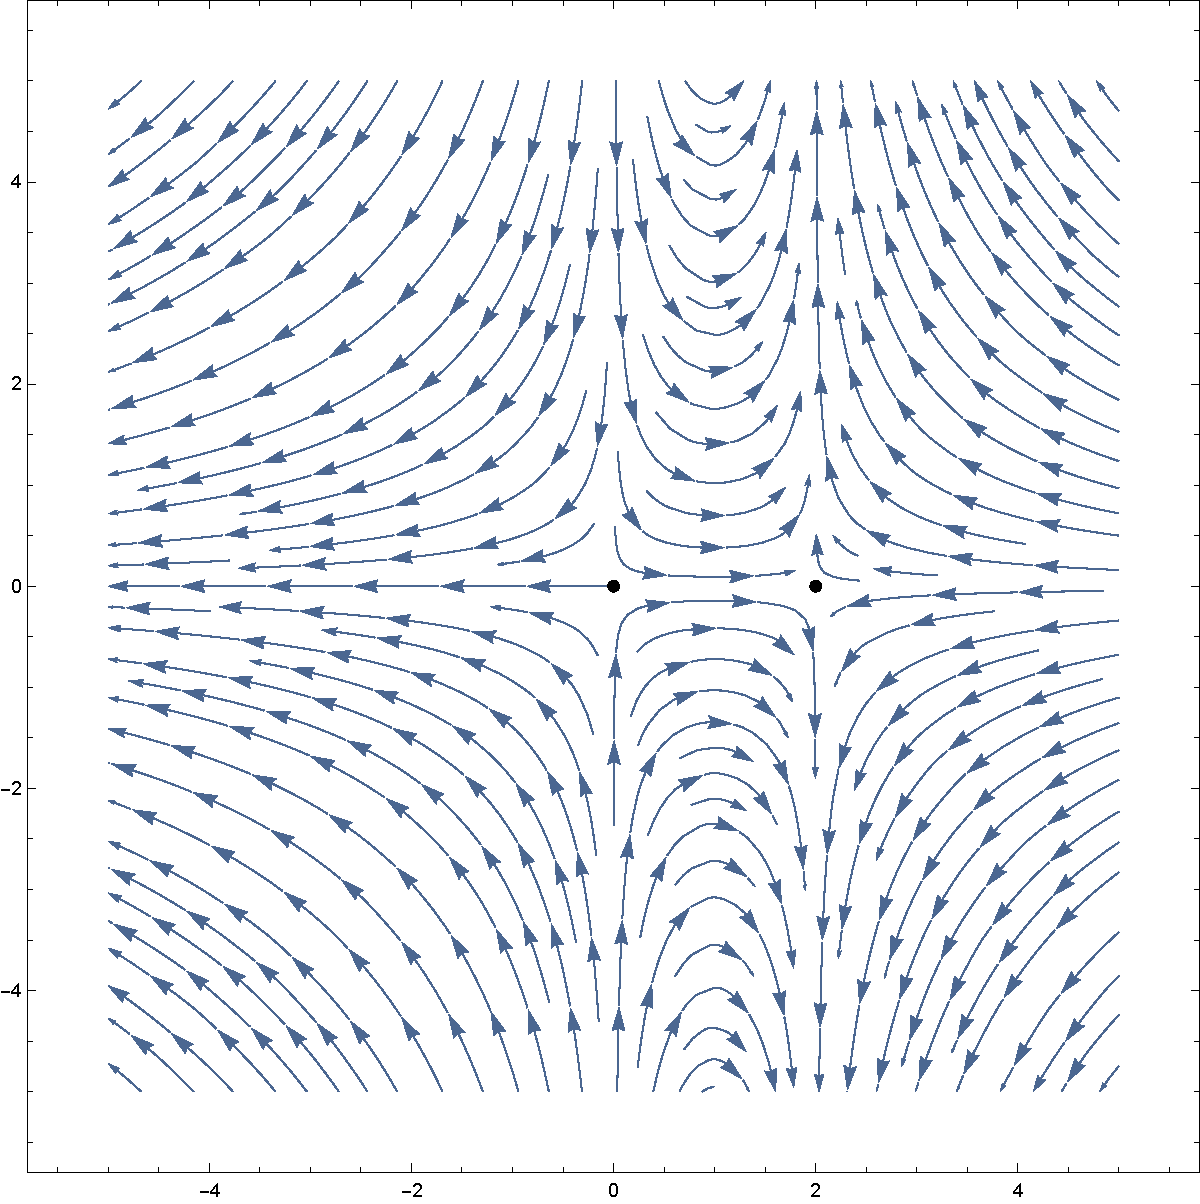
\includegraphics[width=0.8\textwidth]{figures/ex5_vecfComb.pdf}
        \caption{\gr{Διανυσματικό πεδίο συστήματος}}
        \label{fig:ex5_vecfComb}
    \end{figure}

    (β). Μία μη-εγκάρσια τομή στο απλό εκκρεμές είναι η τροχιά που ενώνει τα δύο
    σάγματα. Ελάχιστη μείωση της ενέργειας του εκκρεμούς θα μας πάει στην
    ευσταθή περιοχή, δηλαδή εντός της διαχωριστικής καμπύλης, και αντίστοιχα ελάχιστη
    αύξηση της ενέργειας στη ασταθή, δηλαδή πάνω από τη διαχωριστική καμπύλη.

    Αντίστοιχα είναι τα πράγματα στο σύστημα \tl{Duffing}. Εκεί έχουμε δύο
    περιοχές έλξης και διαχωριστική καμπύλη είναι ο περιστραμμένος κατά
    \( 90 \) αριθμός οκτώ.

    Το να φέρουμε τα συστήματα σε \enquote*{γενική θέση} μπορεί να σημαίνει να
    μεγαλώσουμε την περιοχή όπου τα συστήματα είναι ευσταθή. Ένας τρόπος όπως
    είδαμε είναι με την προσθήκη της απόσβεσης. Θέλουμε όμως να
    παραμείνουμε στην κατηγορία των Χαμιλτονιανών συστημάτων. Η συμπεριφορά των
    Χαμιλτονιανών συστημάτων, του εκκρεμούς και του \tl{Duffing}, θα παραμείνει
    ποιοτικά όπως την περιγράψαμε. Αυτό που μπορούμε να κάνουμε είναι να
    μεγαλώσουμε το χώρο της ευστάθειας. Για παράδειγμα μπορούμε να αλλάξουμε τη συχνότητα
    της ταλάντωσης του εκκρεμούς. Έστω δηλαδή ότι στη συνάρτηση δυναμικού
    όπου \( x \to 0.5x \), τότε θα μεγαλώνουμε το χώρο που είμαστε σε ευστάθεια.
    Αντίστοιχη λογική μπορούμε να ακολουθήσουμε στο σύστημα \tl{Duffing}.
\end{solution}

\begin{exercise}{2016/17 6}
    \emph{Χαμιλτονιανοί πίνακες}: Ο πίνακας γραμμικοποίησης σε σημείο ισορροπίας
    Χαμιλτονιανού συστήματος στο επίπεδο,
    \begin{equation*}
        \dot{x} = \frac{\partial H}{\partial y}, \quad
        \dot{y} = -\frac{\partial H}{\partial x},
    \end{equation*}
    είναι
    \begin{equation*}
        \begin{pmatrix}
            \frac{\partial ^2 H}{\partial x\partial y} &
            \frac{\partial ^2 H}{\partial y^2} \\
            -\frac{\partial ^2 H}{\partial x^2} &
            -\frac{\partial ^2 H}{\partial x\partial y}
        \end{pmatrix},
    \end{equation*}
    και επομένως έχει μηδενικό ίχνος.

    \begin{enumerate}[label= (\alph*)]
        \item Δείξτε ότι η γραμμικοποίηση αυτή δίνει πάντα ή κέντρο ή σάγμα (με
            ίσες σε απόλυτη τιμές ιδιοτιμές).
        \item Ένας τετραγωνικός πίνακας \( A \) διάστασης \( m = 2n \) λέγεται
            \emph{Χαμιλτονιανός} εάν ικανοποιεί την ταυτότητα
            \[
                A^{T}J + JA = 0,
            \]
            όπου \( J \) είναι ο πίνακας
            \begin{equation*}
                \begin{pmatrix}
                    0 &
                    I_n \\
                    -I_n &
                    0
                \end{pmatrix}.
            \end{equation*}
            Δείξτε ότι κάθε τέτοιος \( A \) έχει μηδενικό ίχνος.
        \item Δείξτε ότι εάν \( \lambda \) είναι ιδιοτιμή Χαμιλτονιανού πίνακα
            \( A \), τότε και \( -\lambda \) είναι ιδιοτιμή. (Υπόδειξη: χρήση
                της ορίζουσας της ταυτότητας και θεώρηση του χαρακτηριστικού
            πολυωνύμου.)
        \item Βρείτε τη γενική μορφή Χαμιλτονιανού πίνακα σε δύο διαστάσεις,
            \( m = 2 \), και δείξτε ότι οι ιδιοτιμές του είναι ή \( \lambda =
            \pm i\omega \) ή \( \lambda_2 = -\lambda_1 \).

            Θεωρούμε τώρα μικρές διαταραχές του \( A \) εντός του συνόλου των
            Χαμιλτονιανών πινάκων. Δείξτε ότι εφόσον οι ιδιοτιμές είναι
            μη-μηδενικές, το διαταραγμένο σύστημα έχει σημεία ισορροπίας του
            ίδιου τύπου με το αρχικό (κέντρο ή συμμετρικό σάγμα).
    \end{enumerate}
\end{exercise}
\begin{solution}{2016/17 6}
    (α). Είναι γνωστό ότι χαρακτηριστικό πολυώνυμο στο επίπεδο δίνεται από τη
    σχέση
    \[
        p(\lambda) = \lambda^2 - \lambda\tr{A}+ \det{A},
    \]
    όμως επειδή \( \tr{A} = 0 \) προκύπτει
    \[
        p(\lambda) = \lambda^2 + \det{A}.
    \]
    Επομένως η διακρίνουσα είναι
    \[
        \Delta = -4\det{A}
    \]
    και η λύση
    \begin{equation}\label{eq:ex6_lambda}
        \lambda = \frac{\pm \sqrt{\Delta}}{2}.
    \end{equation}
    Έτσι παίρνουμε περιπτώσεις ανάλογα με την ορίζουσα του \( A \).

    Αν \( \det{A} < 0 \), τότε \( \Delta > 0 \) και άρα οι ιδιοτιμές θα είναι
    πραγματικές με τη μία θετική και την άλλη αρνητική, και φυσικά ίσες σε
    απόλυτη τιμή, όπως φαίνεται στη~\eqref{eq:ex6_lambda}.

    Αν \( \det{A} > 0 \), τότε \( \Delta < 0 \). Όμως επειδή το ίχνος είναι
    μηδέν, δηλαδή το πραγματικό μέρος των ιδιοτιμών είναι μηδέν, αυτό σημαίνει
    ότι θα έχουμε φανταστικές ιδιοτιμές και αυτό συνεπάγεται κέντρο.

    Η περίπτωση όπου \( \det{A} = 0\) δεν έχει νόημα, καθώς τότε μιλάμε για
    μηδενικό πίνακα.

    (β). Αν \( A \) πίνακας διάστασης \( m = 2n \), τότε μπορώ να τον γράψω στη
    μορφή
    \[
        A =
        \begin{pmatrix}
            a & b \\
            c & d
        \end{pmatrix},
    \]
    όπου κάθε μπλοκ \( a, b, c, d \) να είναι ένας \( n \times n \) πίνακας.
    Τότε με αντικατάσταση στην ταυτότητα και αναπτύσσοντας τις πράξεις έχουμε
    \begin{align*}
        A^{T}J + JA &=
        \begin{pmatrix}
            a & c \\
            b & d
        \end{pmatrix}
        \begin{pmatrix}
            0 & I_n \\
            -I_n & 0
        \end{pmatrix} +
        \begin{pmatrix}
            0 & I_n \\
            -I_n & 0
        \end{pmatrix}
        \begin{pmatrix}
            a & b \\
            c & d
        \end{pmatrix} \\
        &=\begin{pmatrix}
            -cI_n & aI_n \\
            -dI_n & bI_n
        \end{pmatrix} +
        \begin{pmatrix}
            I_{n}c & I_{n}d \\
            -I_{n}a & -I_{n}b
        \end{pmatrix}\\
        &=\begin{pmatrix}
            -cI_n + I_{n}c & aI_n + I_{n}d\\
            -dI_n - I_{n}a & bI_n -I_{n}b
        \end{pmatrix} \\
        &=\begin{pmatrix}
            0 & aI_n + I_{n}d\\
            -dI_n - I_{n}a & 0
        \end{pmatrix}.
    \end{align*}
    Όμως για να ισχύει η ταυτότητα θα πρέπει να ισχύει για τους πίνακες
    \( a \) και \( d \)
    \[
        a + d = 0,
    \]
    και άρα ο πίνακας \( A \) θα έχει μηδενικό ίχνος. Έτσι ο πίνακας \( A \)
    μπορεί να γραφτεί στη μορφή
    \[
        A =
        \begin{pmatrix}
            a & b \\
            c & -a
        \end{pmatrix}.
    \]

    (γ). Αρχικά παρατηρούμε ότι
    \[
        -J = \begin{pmatrix}
            0 & -I_n \\
            I_n & 0
        \end{pmatrix} = J^T,
    \]
    που σημαίνει ότι
    \[
        J^{T}J = (-J) (-J^T) = JJ^T =
        \begin{pmatrix}
            0 & I_n \\
            -I_n & 0
        \end{pmatrix}
        \begin{pmatrix}
            0 & -I_n \\
            I_n & 0
        \end{pmatrix} = I_m.
    \]
    Το παραπάνω σημαίνει πως \( J^T = J^{-1} \), δηλαδή ο \( J \) είναι ορθογώνιος
    πίνακας και συνεπώς οι ιδιοτιμές του είναι \( \pm 1 \). Πιο συγκεκριμένα, οι
    ιδιοτιμές του \( J \) είναι
    \[
        \det{J} = \det{\begin{pmatrix}0 & I_n\\ -I_n & 0\end{pmatrix}} =
        \det{\left( 0 - (-I_n)I_n \right)} = \det{I_n} = 1.
    \]

    Από την ταυτότητα των Χαμιλτονιανών πινάκων έχουμε
    \begin{align*}
        0 &= A^{T}J + JA \\
        -JA &= A^{T}J \\
        -A &= J^{-1}A^{T}J \\
        -A &= -JA^{T}J \\
        A &= JA^{T}J.
    \end{align*}

    Τώρα αν πάρουμε το χαρακτηριστικό πολυώνυμο του \( A \) προκύπτει
    \begin{align*}
        p(\lambda) &= \det{\left( A - \lambda I_m \right)}
        = \det{\left( JA^{T}J - \lambda J^{T}J \right)} \\
        &= \det{\left( JA^{T}J + \lambda J^{2} \right)}
        = \det{\left( J\left(A^{T} + \lambda I_m\right)J \right)} \\
        &= \det{\left( J \right)}
        \det{\left( A^T + \lambda I_m \right)}
        \det{\left( J \right)}\\
        &= \det{\left( A^T + \lambda I_m \right)}
        = \det{\left( A + \lambda I_m \right)^{T}}\\
        &= \det{\left( A + \lambda I_m \right)}
        = \det{\left( A - (-\lambda) I_m \right)}\\
        &= p(-\lambda).
    \end{align*}

    (δ). Άμεσα από τα παραπάνω έχουμε ότι αν \( \lambda \) είναι η μία ιδιοτιμή
    του \( A \) τότε η \( -\lambda \) θα είναι η άλλη ιδιοτιμή του. Αν \( A \)
    είναι δισδιάστατος πίνακας της μορφής
    \[
        A =
        \begin{pmatrix}
            a & b \\
            c & d
        \end{pmatrix},
    \]
    τότε θα ισχύει
    \begin{align*}
        \det{\begin{pmatrix}
                a - \lambda & b \\
                c & d - \lambda
        \end{pmatrix}} &=
        \det{\begin{pmatrix}
                a + \lambda & b \\
                c & d + \lambda
        \end{pmatrix}} \\
        (a - \lambda)(d - \lambda) - bc &=
        (a + \lambda)(d + \lambda) - bc \\
        ad - a\lambda - \lambda d + \lambda^2 &=
        ad + a\lambda + \lambda d + \lambda^2,
    \end{align*}
    που συνεπάγεται
    \[
        \lambda(a + d) = 0,
    \]
    και άρα \( \lambda = 0 \) ή στη γενικά \( d = -a \). Επομένως ο \( A \) έχει
    μηδενικό ίχνος και είναι της γενικής μορφής
    \[
        A =
        \begin{pmatrix}
            a & b \\
            c & -a
        \end{pmatrix}.
    \]
    Το χαρακτηριστικό πολυώνυμο του \( A \) είναι
    \[
        p(\lambda) = \lambda^2 + \det{A},
    \]
    με διακρίνουσα \( \Delta = -4 \det{A} \). Σύμφωνα με την ανάλυση που κάναμε
    στο ερώτημα (α), καταλήγουμε ότι οι ιδιοτιμές του πίνακα \( A \) είναι \(
    \lambda = \pm i\omega \) ή \( \lambda_2 = - \lambda_1 \).

    Σύμφωνα με τα παραπάνω, οι ιδιοτιμές του \( A \) θα είναι διακριτές.
    Συνεπώς, αν πάρουμε τη μορφή \tl{Jordan} του \( A \) στο χώρο \(
    M_n\left(\mathbb{C}\right) \) τότε θα οι ιδιοτιμές θα είναι τα διαγώνια
    στοιχεία. Αν τώρα διαταράξουμε \enquote*{λίγο} τα στοιχεία αυτά, τότε οι
    συντελεστές του χαρακτηριστικού πολυωνύμου του \( A \) θα διαταραχθούν
    \enquote*{λίγο}. Έτσι οι ρίζες του πολυωνύμου θα διαταραχθούν
    \enquote*{λίγο}. Συνεπώς, εφόσον ο πίνακας \( A \) έχει διακριτές ιδιοτιμές,
    πίνακες αυθαίρετα κοντά σε αυτόν θα έχουν τις ίδιες ιδιότητες με τον
    \( A \), και άρα τα σημεία ισορροπίας θα είναι του ίδιου τύπου με το αρχικό.
\end{solution}

\begin{exercise}{2016/17 7}
    \emph{Βέλτιστος έλεγχος και Χαμιλτονιανά συστήματα}: Συνοπτικά, εάν έχουμε
    αφινικό σύστημα ελέγχου
    \[
        \dot{x} = f(x) + g(x)u, \quad x \in \mathbb{R}^n, u \in \mathbb{R}^m,
    \]
    με \( g(x) n \times m \) πίνακα σταθερού βαθμού \( m \) και θεωρήσουμε
    συναρτησιακό κόστους με \tl{Lagrangian} \( L(x, u) \) (θετικά ορισμένη στο
    \( u \)), σχηματίζουμε την Χαμιλτονιανή
    \[
        H(x, u, p) = \left( f(x) + g(x)u \right)\cdot p - L(x, u),
    \]
    όπου \( p \in \mathbb{R}^n \) δυϊκές μεταβλητές
    (\enquote*{πολλαπλασιαστές \tl{Lagrange}}).

    Η αρχή μεγίστου (ή ελαχίστου) του \tl{Pontryagin} οδηγεί στη βέλτιστη
    Χαμιλτονιανή
    \[
    H^*(x, p) = \underset{u}\sup \, H(x, u, p).
    \]
    Συνήθως, αυτό μας δίνει τον βέλτιστο έλεγχο ως συνάρτηση των \( x \) και
    \( p, u^*(x, p) \). Εάν κάποιες επιπλέον συνθήκες ισχύουν, τότε οι βέλτιστες
    λύσεις \( (x(t), p(t)) \) είναι οι τροχιές του Χαμιλτονιανού συστήματος για
    τη συνάρτηση \( H^* \).
    \begin{enumerate}[label= (\alph*)]
        \item Βρείτε τον βέλτιστο έλεγχο \( u^* \) και την \( H^* \) για
            γραμμικά συστήματα,
            \[
                \dot{x} = Ax + Bu, \quad \rank{B} = m
            \]
            και για \tl{Lagrangian}
            \[
                L(x, u) = \frac{1}{2}x^{T}Rx + \frac{1}{2}u^{T}Qu, \quad R \geq
                0, Q >0
            \]
            και δώστε τις Χαμιλτονιανές του εξισώσεις (που πρέπει να είναι
            γραμμικές!).
        \item Μελετήστε το σύστημα σε μία διάσταση \( \dot{x} = ax + bu (b \neq
            0) \) και βρείτε τις λύσεις \( (x, p) \) για την ασταθή περίπτωση \(
            a > 0 \).
    \end{enumerate}
\end{exercise}
\begin{solution}
    (α). Για να συμβαδίσω με τους συμβολισμούς που έχω συνηθίσει μέχρι τώρα θα ορίσω
    τη \tl{Lagrangian} ως
    \[
        L(x, u) = \frac{1}{2}x^{T}Qx + \frac{1}{2}u^{T}Ru, \quad Q \geq
        0, R > 0,
    \]
    δηλαδή θα αλλάξω το \( Q \) με το \( R \) και θα ακολουθήσουμε τη διαδικασία
    για την αρχή του ελαχίστου.

    Θεωρούμε την επαυξημένη \tl{Lagrangian}
    \begin{align}\label{eq:ex7_aug_lag}
        L_a(x, u) &= L(x, u) + p^T\left( Ax + Bu - \dot{x} \right) \nonumber \\
        &= \frac{1}{2}x^{T}Qx + \frac{1}{2}u^{T}Ru + p^T\left( Ax + Bu - \dot{x}
        \right).
    \end{align}
    Από το λογισμό των μεταβολών είναι γνωστό ότι, οι αναγκαίες συνθήκες για την
    ύπαρξη ακρότατου είναι να ικανοποιούνται οι εξισώσεις \tl{Euler-Lagrange}.
    Έτσι για τη σχέση~\eqref{eq:ex7_aug_lag} πρέπει να ισχύει
    \begin{align}
        0 &= \frac{\partial L_a}{\partial p}(x^*, u^*, p^*) -
        \frac{d}{dt}\left(
        \frac{\partial L_a}{\partial \dot{p}}(x^*, u^*, p^*)\right)
        \label{eq:ex7_eul_lag_p}\\
        0 &= \frac{\partial L_a}{\partial x}(x^*, u^*, p^*) -
        \frac{d}{dt}\left(
        \frac{\partial L_a}{\partial \dot{x}}(x^*, u^*, p^*)\right)
        \label{eq:ex7_eul_lag_x}\\
        0 &= \frac{\partial L_a}{\partial u}(x^*, u^*, p^*) -
        \frac{d}{dt}\left(
        \frac{\partial L_a}{\partial \dot{u}}(x^*, u^*, p^*)\right).
        \label{eq:ex7_eul_lag_u}
    \end{align}
    Ορίζουμε την Χαμιλτονιανή ως
    \begin{align}\label{eq:ex7_hamilton}
        H(x, u, p) &= L(x, u) + p^T\left(Ax + Bu\right) \nonumber \\
        &= \frac{1}{2}x^{T}Qx + \frac{1}{2}u^{T}Ru + p^T\left( Ax + Bu \right).
    \end{align}
    Με αντικατάσταση της \( L(x, u) \) από τη σχέση~\eqref{eq:ex7_aug_lag}
    \[
        L(x ,u) = L_a(x, u, p) - p^T\left(Ax + Bu - \dot{x} \right),
    \]
    θα έχουμε
    \[
        H(x, u, p) = L_a(x, u, p) - p^T\left( Ax + Bu - \dot{x} \right)
        + p^T\left( Ax + Bu \right),
    \]
    και τελικά προκύπτει
    \[
        L_a(x, u, p) = H(x, u, p) - p^{T}\dot{x}.
    \]
    Έτσι από τη σχέση~\eqref{eq:ex7_eul_lag_p} προκύπτει
    \begin{align*}
        0 &= \frac{\partial H(x^*, u^*, p^*) - p^{T}\dot{x}}{\partial p} -
        \frac{d}{dt}\left(
        \frac{\partial H(x^*, u^*, p^*) - p^{T}\dot{x}}{\partial \dot{p}}\right)
        \\
        0 &= \frac{\partial H}{\partial p} (x^*, u^*, p^*) - \dot{x},
    \end{align*}
    που οδηγεί στη σχέση
    \begin{equation}\label{eq:ex7_Hx_star}
        \dot{x}^* = \frac{\partial H}{\partial p} (x^*, u^*, p^*).
    \end{equation}
    Αντίστοιχα από τη σχέση~\eqref{eq:ex7_eul_lag_x} προκύπτει
    \begin{align*}
        0 &= \frac{\partial H(x^*, u^*, p^*) - p^{T}\dot{x}}{\partial x} -
        \frac{d}{dt}\left(
        \frac{\partial H(x^*, u^*, p^*) - p^{T}\dot{x}}{\partial \dot{x}}\right)
        \\
        0 &= \frac{\partial H}{\partial x} (x^*, u^*, p^*) - \frac{d}{dt}(-p),
    \end{align*}
    που οδηγεί στη σχέση
    \begin{equation}\label{eq:ex7_Hp_star}
        \dot{p}^* = -\frac{\partial H}{\partial x} (x^*, u^*, p^*).
    \end{equation}
    Τέλος, από τη σχέση~\eqref{eq:ex7_eul_lag_x} προκύπτει
    \[
        0 = \frac{\partial H(x^*, u^*, p^*) - p^{T}\dot{x}}{\partial u} -
        \frac{d}{dt}\left(
        \frac{\partial H(x^*, u^*, p^*) - p^{T}\dot{x}}{\partial \dot{u}}\right)
    \]
    που οδηγεί στη σχέση
    \begin{equation}\label{eq:ex7_Hu_star}
        0 = \frac{\partial H}{\partial u} (x^*, u^*, p^*).
    \end{equation}

    Από τη σχέση~\eqref{eq:ex7_Hu_star} προκύπτει
    \begin{align*}
        0 &= \frac{\partial H}{\partial u} (x^*, u^*, p^*) \\
        &= Ru^* + B^{T}p^*,
    \end{align*}
    που οδηγεί στον βέλτιστο έλεγχο
    \begin{equation}\label{eq:ex7_u_star}
        u^* = -R^{-1}B^{T}p^*.
    \end{equation}
    Από τη σχέση~\eqref{eq:ex7_Hp_star} προκύπτει
    \begin{align}\label{eq:ex7_p_star}
        \dot{p}^* &= -\frac{\partial H}{\partial x} (x^*, u^*, p^*) \nonumber \\
        \dot{p}^* &= -\left(Qx^* + A^{T}p^*\right) \nonumber \\
        \dot{p}^* &= -Qx^* - A^{T}p^*.
    \end{align}
    Από τη σχέση~\eqref{eq:ex7_Hx_star} προκύπτει
    \begin{align}\label{eq:ex7_x_star}
        \dot{x}^* &= \frac{\partial H}{\partial p} (x^*, u^*, p^*) \nonumber \\
        \dot{x}^* &= Ax^* + Bu^*,
    \end{align}
    που οδηγεί στους περιορισμούς του προβλήματος. Με αντικατάσταση
    της~\eqref{eq:ex7_u_star} στην~\eqref{eq:ex7_x_star} προκύπτει
    \[
        \dot{x}^* = Ax^* - BR^{-1}B^{T}p^*.
    \]
    Από την παραπάνω σε συνδυασμό με τη σχέση~\eqref{eq:ex7_p_star} προκύπτει
    ένα σύστημα γραμμικών κανονικών διαφορικών πρώτης τάξης ως προς
    \( x^* \) και \( p^* \)
    \begin{equation}\label{eq:ex7_xp_sys}
        \begin{pmatrix}
            \dot{x}^* \\
            \dot{p}^*
        \end{pmatrix} =
        \begin{pmatrix}
            A & -BR^{-1}B^{T} \\
            -Q & -A^{T}
        \end{pmatrix}
        \begin{pmatrix}
            x^* \\
            p^*
        \end{pmatrix}.
    \end{equation}
    Επίλυση του παραπάνω συστήματος~\eqref{eq:ex7_xp_sys} καθώς και από τη
    σχέση~\eqref{eq:ex7_u_star} βρίσκουμε τις βέλτιστες καταστάσεις, τους
    βέλτιστους πολλαπλασιαστές \tl{Lagrange} καθώς και το βέλτιστο έλεγχο,
    αντίστοιχα. Τέλος, με αντικατάσταση αυτών στη σχέση της
    Χαμιλτονιανής~\eqref{eq:ex7_hamilton}, προκύπτει η βέλτιστη τιμή της \( H^*
    \).

    (β). Θα εφαρμόσουμε τα παραπάνω στο σύστημα \( \dot{x} = ax + bu \) με \( a >
    0 \) και \( b \neq 0 \). Έτσι η Χαμιλτονιανή θα είναι
    \[
        H(x, u, p) = \frac{1}{2}qx^2 + \frac{1}{2}ru^2 + p(ax + bu).
    \]
    Ο βέλτιστος έλεγχος θα είναι
    \[
        u^* = -\frac{b}{r}p^*.
    \]
    Για να βρω το βέλτιστο έλεγχο θα πρέπει να λύσω το σύστημα
    \begin{equation*}
        \begin{pmatrix}
            \dot{x}^* \\
            \dot{p}^*
        \end{pmatrix} =
        \begin{pmatrix}
            a & -\frac{b^2}{r} \\
            -q & -a
        \end{pmatrix}
        \begin{pmatrix}
            x^* \\
            p^*
        \end{pmatrix} = A
        \begin{pmatrix}
            x^* \\
            p^*
        \end{pmatrix}.
    \end{equation*}
    Ένας τρόπος για να βρούμε τις οριακές συνθήκες είναι ο εξής. Αν επιθυμούμε
    η κατάσταση \( x \) να πάει στο μηδέν στο τελικό χρόνο, τότε
    για γνωστή αρχική συνθήκη και καθορισμένο τελικό χρόνο, μπορούμε να
    υπολογίσουμε την αρχική συνθήκη για τον πολλαπλασιαστή \tl{Lagrange}. Έτσι
    λύση της παραπάνω για τελικό χρόνο \( t_f \) είναι
    \begin{equation*}
        \begin{pmatrix}
            x^*(t_f) \\
            p^*(t_f)
        \end{pmatrix} =
        e^{At_f}
        \begin{pmatrix}
            x(t_0) \\
            p(t_0)
        \end{pmatrix} =
        \begin{pmatrix}
            h & j \\
            k & l
        \end{pmatrix}
        \begin{pmatrix}
            x(t_0) \\
            p(t_0)
        \end{pmatrix}.
    \end{equation*}
    Άρα η πρώτη σχέση από το παραπάνω σύστημα δίνει
    \[
        x^*(t_f) = hx_0 + j p_0,
    \]
    που σημαίνει
    \[
        p_0 = \frac{x^*(t_f) - hx_0}{j}.
    \]

    Το σύστημα διότι είναι σε μικρές διαστάσεις έχει αναλυτική λύση που θα
    γράψουμε παρακάτω. Γενικά, αναλυτικές λύσεις δεν μπορούμε να βρούμε, παρά
    μόνο όταν είναι τόσο απλά συστήματα.
    \begin{align*}
        x^*(t) &= \frac{
            \sqrt{r}wc_2\cosh{vt} + (b^2c_1 + arc_2)\sinh{vt}
        }{\sqrt{r}w} \\
        p^*(t) &= \frac{
            wc_1\cosh{vt} - \sqrt{r}(ac_1 + qc_2)\sinh{vt}
        }{w},
    \end{align*}
    όπου \( c_1, c_2 \) είναι οι σταθερές ολοκλήρωσης και υπολογίζονται από τις
    οριακές συνθήκες και \(w, v \) είναι
    \[
        w = \sqrt{b^2q + a^2r}, \quad v = \sqrt{\frac{b^2q + a^2r}{r}}.
    \]

    Στο σχήμα~\ref{fig:ex7_case1} βλέπουμε μία λύση του συστήματος. Οι
    παράμετροι έχουν επιλεγεί ως \( a = 2, b = 1, q = 1, r = 0.25 \), ακόμη η
    αρχική συνθήκη για το \( x_0 = 5 \) και επιθυμούμε η κατάσταση να φτάσει στο
    μηδέν.
    \begin{figure}[h]
        \centering
        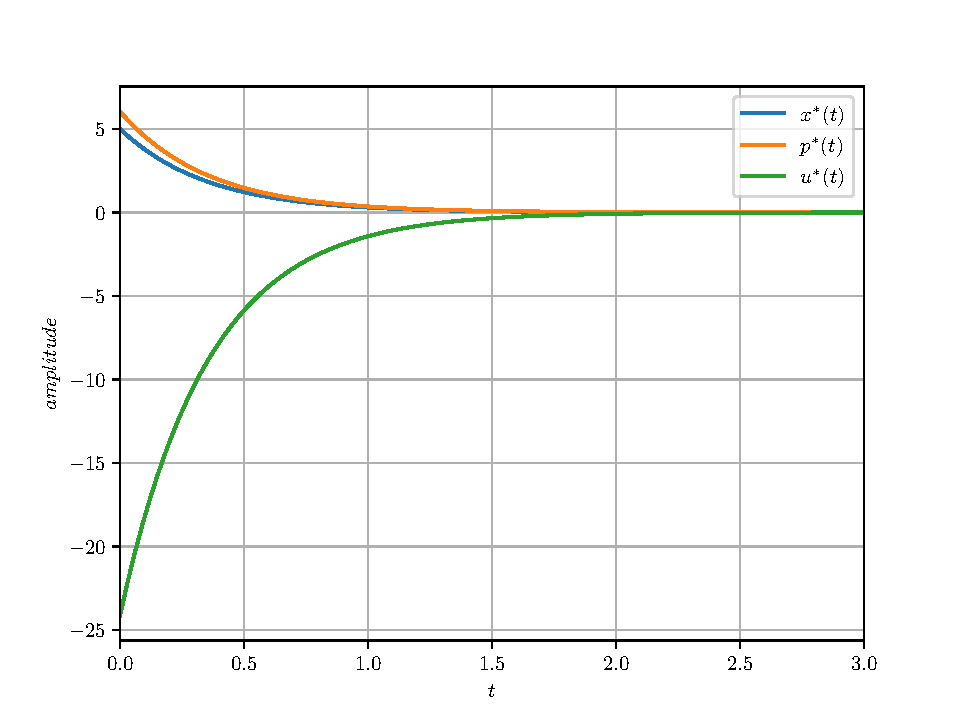
\includegraphics[width=0.9\textwidth]{figures/ex7_case1.pdf}
        \caption{\gr{Βέλτιστες τροχιές,
        \( a = 2, b = 1, q = 1, r = 0.25 \)}}
        \label{fig:ex7_case1}
    \end{figure}
\end{solution}


\begin{exercise}{2016/17 9}
    Εξετάστε το ακόλουθο πρόβλημα: δίνεται γραμμικό υποψήφιο σύστημα
    \( \dot{x} = Ax \) στο \( \mathbb{R}^n \), με το \( 0 \) ασυμπτωτικά
    ευσταθές. Η απλούστερη μορφή υποψήφιας συνάρτησης \tl{Lyapunov} για το \( 0
    \) είναι
    \[
        V(x) = \frac{1}{2}x^{T}Qx,
    \]
    με \( Q = Q^T > 0 \) (θετικά ορισμένο, συμμετρικό). Γιατί;

    Δείξτε ότι πάντα υπάρχει τέτοιος \( Q \) και μάλιστα με \( \frac{dV}{dt} =
    -x^{T}Px \), με \( P \) επίσης θετικά ορισμένο συμμετρικό πίνακα.

    Δώστε ένα (μη-διαγώνιο!) παράδειγμα στο \( \mathbb{R}^3 \).
\end{exercise}
\begin{solution}
    Για να είναι η \( V \) συνάρτηση \tl{Lyapunov} στο \( 0 \) θα πρέπει να
    ικανοποιούνται τα παρακάτω. Πρώτον, προφανώς στο \( 0 \) ισχύει
    \[
        V(0) = 0.
    \]
    Δεύτερον, για κάθε \( x \neq 0 \) ισχύει ότι
    \[
        V(x) = \frac{1}{2}x^{T}Qx > 0,
    \]
    διότι \( Q \) είναι θετικά ορισμένος και συμμετρικός. Τρίτον, για \( x \neq
    0 \) ισχύει ότι
    \[
        \frac{dV}{dt} = \frac{1}{2}
        \frac{\partial \left( x^{T}Qx \right)}{\partial x}
        \frac{dx}{dt} =
        x^{T}QAx.
    \]
    Όμως γνωρίζουμε πως το \( 0 \) είναι ασυμπτωτικά ευσταθές. Ακόμα, επειδή το
    σύστημα είναι γραμμικό, αυτό συνεπάγεται πως ο πίνακας \( A \) θα είναι
    αρνητικά ορισμένος. Έτσι το γινόμενο του θετικά ορισμένου \( Q \) με τον
    αρνητικά ορισμένο \( A \) θα μας δώσει έναν αρνητικά ορισμένο πίνακα.
    Άρα ισχύει
    \[
        \frac{dV}{dt} = x^{T}QAx < 0,
    \]
    για κάθε \( x \neq 0 \). Τέτοιος \( Q \) υπάρχει πάντα καθώς η ευστάθεια του
    \( 0 \) εξαρτάται αποκλειστικά από τον πίνακα \( A \). Ακόμα το γινόμενο
    \( QA \) μπορεί να γραφτεί σαν ένας πίνακας \( P \) που θα είναι θετικά
    ορισμένος και έτσι η παραπάνω σχέση μπορεί να γραφτεί
    \[
        \frac{dV}{dt} = -x^{T}Px.
    \]
    Ένα τέτοιο παράδειγμα στο \( \mathbb{R}^3 \) είναι το παρακάτω. Ο \( Q \)
    είναι
    \[
        Q =
        \begin{pmatrix}
            2 & -1 & 0 \\
            -1 & 2 & -1 \\
            0 & -1 & 2
        \end{pmatrix},
    \]
    που έχει ιδιοτιμές \( \lambda_1 = 3.4141, \lambda_2 = 2, \lambda_3 = 0.5857
    \) και άρα είναι θετικά ορισμένος. Ο \( P \) είναι
    \[
        P =
        \begin{pmatrix}
            2 & -1 & 1 \\
            -1 & 2 & -1 \\
            1 & -1 & 2
        \end{pmatrix},
    \]
    που έχει ιδιοτιμές \( \lambda_1 = 1, \lambda_2 = 4, \lambda_3 = 1 \), που
    επίσης έχει θετικές ιδιοτιμές και άρα είναι θετικά ορισμένος. Ο πίνακας
    \( A \) είναι
    \[
        A =
        \begin{pmatrix}
            -1.25 & 0 & -0.75 \\
            -0.5 & -1 & -0.5 \\
            -0.75 & 0 & -1.25
        \end{pmatrix},
    \]
    που έχει ιδιοτιμές \( \lambda_1 = -1, \lambda_2 = -0.5, \lambda_3 = -2 \), που
    έχει αρνητικές ιδιοτιμές και άρα είναι αρνητικά ορισμένος.
\end{solution}

\begin{exercise}{2016/17 10}
    \emph{Σταθεροποίηση του σαγματικού σημείου του εκκρεμούς}: Θα αναλύσουμε
    κάποιες μεθόδους \enquote*{εξισορρόπησης} του εκκρεμούς στην κάθετη προς τα
    πάνω θέση (χωρίς να ισχυριζόμαστε ότι είναι ιδιαίτερα χρήσιμες στην πράξη).

    Οι εξισώσεις είναι, όπως και πριν:
    \begin{align*}
        \dot{x} &= y \\
        \dot{y} &= -a y - \sin{x}
    \end{align*}
    για \( a \) θετικό και μικρό (π.χ. \( a = 0.3 \)).
    \begin{enumerate}[label= (\alph*)]
        \item Θεωρούμε έλεγχο που επεισέρχεται στην εξίσωση για τη γωνία, δηλαδή
            θεωρούμε τη νέα πρώτη εξίσωση:
            \[
                \dot{x} = y + u_1(x).
            \]
            Βρείτε τον έλεγχο \( u_1(x) = -kx + c \) ο οποίος σταθεροποιεί το
            σαγματικό σημείο \( (x, y) = (\pi, 0) \), δηλαδή να έχει το σημείο
            αυτό ως ολικό ελκυστή (ασυμπτωτικά ευσταθές σημείο ισορροπίας).
            Είναι δυνατό αυτό εάν το σύστημα είναι χωρίς απώλειες
            (δηλαδή \( a = 0 \));
        \item Επαναλάβετε για έλεγχο στη γωνιακή ταχύτητα, δηλαδή με νέα δεύτερη
            εξίσωση:
            \[
                \dot{y} = -ay -\sin{x} + u_2(x),
            \]
            πάλι με \( u_2(x) = -kx + c \).
    \end{enumerate}
    Και στις δύο περιπτώσεις, δώστε κατάλληλα πορτρέτα κίνησης του ελεγχόμενου
    συστήματος που επιλέξατε.
\end{exercise}
\begin{solution}
    (α). Με τον έλεγχο \( u_1(x) \) οι εξισώσεις είναι
    \begin{align*}
        \dot{x} &= y -kx + c\\
        \dot{y} &= -a y - \sin{x}.
    \end{align*}
    Εφόσον θέλουμε το σημείο \( (\pi, 0) \) να είναι ασυμπτωτικά ευσταθές,
    μπορούμε από τη γραμμικοποίηση να βρούμε τις συνθήκες για το \( k \) που θα
    επιτυγχάνει το στόχο αυτόν. Έτσι έχουμε
    \[
        \begin{pmatrix}
            \dot{x} \\
            \dot{y}
        \end{pmatrix} = F(x, y) =
        \begin{pmatrix}
            y -kx + c \\
            -a y - \sin{x}
        \end{pmatrix}.
    \]
    Η γραμμικοποίηση είναι
    \[
        DF(x, y) =
        \begin{pmatrix}
            -k & 1 \\
            -\cos{x} & -a
        \end{pmatrix},
    \]
    και στο σημείο \( (\pi, 0) \) έχουμε
    \[
        DF(\pi, 0) =
        \begin{pmatrix}
            -k & 1 \\
            1 & -a
        \end{pmatrix}.
    \]
    Εφόσον θέλουμε ασυμπτωτική ευστάθεια, θα πρέπει \(
    \operatorname{Re}(\lambda) < 0 \). Άρα οι ιδιοτιμές είναι
    \begin{align*}
        \det{\begin{pmatrix}
                -k - \lambda & 1 \\
                1 & -a - \lambda
        \end{pmatrix}} &=
        (-k - \lambda)(-a - \lambda) - 1 \\
        &= ka + k\lambda + \lambda a + \lambda^2 - 1 \\
        &= \lambda^2 + \lambda(k + a) + ka - 1.
    \end{align*}
    Η διακρίνουσα της παραπάνω είναι
    \begin{align*}
        \Delta &= (k + a)^2 - 4(ka - 1) \\
        &= k^2 + a^2 + 2ka - 4ka + 4 \\
        &= (k - a)^2 + 4 > 0.
    \end{align*}
    Συνεπώς, έχουμε δύο διακριτές πραγματικές ιδιοτιμές. Επομένως πρέπει
    \[
        \lambda = \frac{-(k + a) \pm\sqrt{(k -a)^2 + 4}}{2} < 0.
    \]
    Έστω \( \lambda_1 \) η ιδιοτιμή που αντιστοιχεί όταν μπροστά από την
    τετραγωνική ρίζα έχουμε το θετικό πρόσημο και \( \lambda_2 \) η ιδιοτιμή
    που αντιστοιχεί όταν μπροστά από την τετραγωνική ρίζα έχουμε το αρνητικό
    πρόσημο.

    Οι ρίζες της \( \lambda_1 \) είναι
    \[
        -(k + a) + \sqrt{(k -a)^2 + 4} = 0,
    \]
    που συνεπάγεται
    \begin{align*}
         \sqrt{(k -a)^2 + 4} &= (k + a) \\
         (k -a)^2 + 4 &= (k + a)^2 \\
         k^2 + a^2 -2ka + 4 &= k^2 + a^2 + 2ka \\
         -4ka &= -4 \\
         k &= \frac{1}{a}. \\
    \end{align*}
    Άρα για την ιδιοτιμή \( \lambda_1 \) πρέπει
    \begin{equation}\label{eq:ex10_a_lambda_1}
        \lambda_1 < 0 \Rightarrow k > \frac{1}{a}.
    \end{equation}
    Ομοίως για την ιδιοτιμή \( \lambda_2 \) πρέπει
    \[
        -(k + a) - \sqrt{(k -a)^2 + 4} < 0,
    \]
    που όμως αρκεί
    \begin{align*}
        -(k + a) &< 0 \\
        -k &< a.
    \end{align*}
    Άρα για την ιδιοτιμή \( \lambda_2 \) πρέπει
    \[
        \lambda_2 < 0 \Rightarrow k > -a,
    \]
    η οποία όμως είναι περιττή καθώς εμπεριέχεται από την ανισότητα της
    σχέσης~\eqref{eq:ex10_a_lambda_1}.

    Δηλαδή για \( k > 1/a \) και οριακά για \( k = 1/a \) το σύστημα, η
    συνιστώσα \( x \) (θέση), θα ισορροπήσει στο σαγματικό σημείο ισορροπίας
    \( (\pi, 0) \) το οποίο θα είναι ασυμπτωτικά ευσταθές. Το πόσο γρήγορα θα
    φτάσουμε στο στόχο μας εξαρτάται από την απόλυτη τιμή των ιδιοτιμών. Έτσι
    για \( k = 1/a \) θα φτάσουμε το στόχο, αλλά \enquote*{αργά}. Όσο αυξάνεται
    το \( k \) τόσο πιο γρήγορα θα ισορροπήσει η θέση στη γωνία \( \pi \).

    Από τη συνθήκη για το \( k \), η ανισότητα της
    σχέσης~\eqref{eq:ex10_a_lambda_1}, φαίνεται ότι όσο μικραίνει η απόσβεση,
    τόσο μεγαλύτερο πρέπει να γίνει το \( k \). Για την οριακή τιμή \( a = 0 \)
    τότε \( k \to \infty \) και άρα το να ισορροπήσουμε το σύστημα στη θέση \(
    (\pi, 0) \) είναι αδύνατο.

    Στο σχήμα~\ref{fig:ex10_invPend15a} παρουσιάζεται η χρονική απόκριση του
    εκκρεμούς με αρχικές συνθήκες \( (0, 0) \), για μικρή απόσβεση \( a = 0.3 \)
    και έλεγχο
    \[
        u_1(x) = -\frac{1.5}{a}x + \frac{1.5}{a}\pi.
    \]
    Το μικρό κέρδος όπως βλέπουμε, παρόλο που καταφέρνει να ισορροπήσει το
    σύστημα στο \( (\pi, 0) \) απαιτεί πολύ χρόνο.
    \begin{figure}[h!]
        \centering
        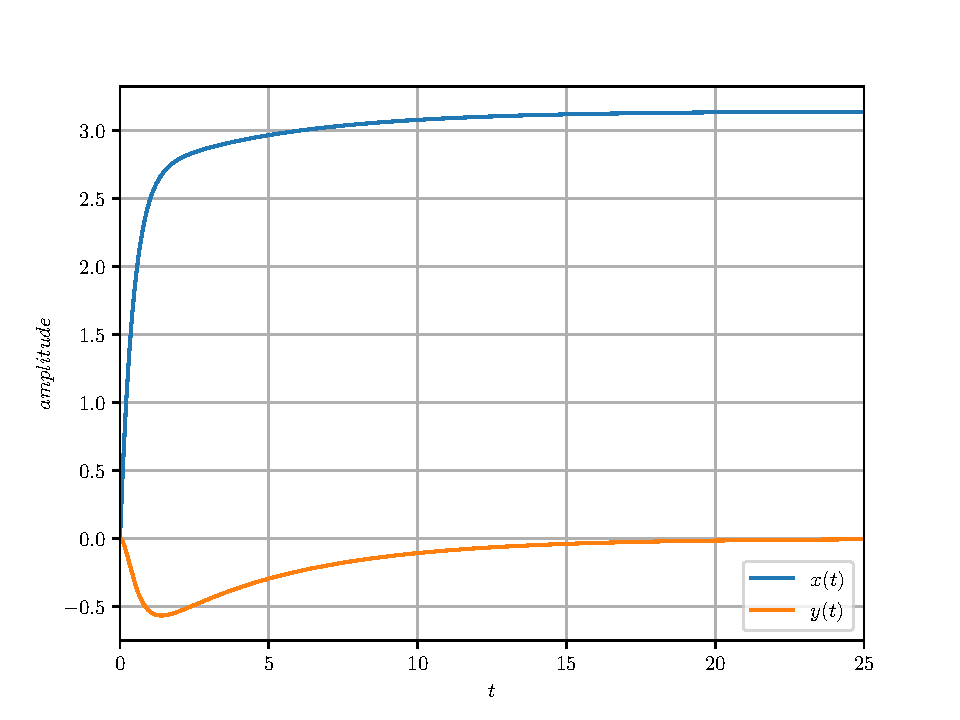
\includegraphics[width=0.9\textwidth]{figures/ex10_invPend15a.pdf}
        \caption{\gr{Χρονική απόκριση ανάστροφου εκκρεμούς,
        \( k = 1.5/a, a = 0.3 \)}}
        \label{fig:ex10_invPend15a}
    \end{figure}
    \begin{figure}[h!]
        \centering
        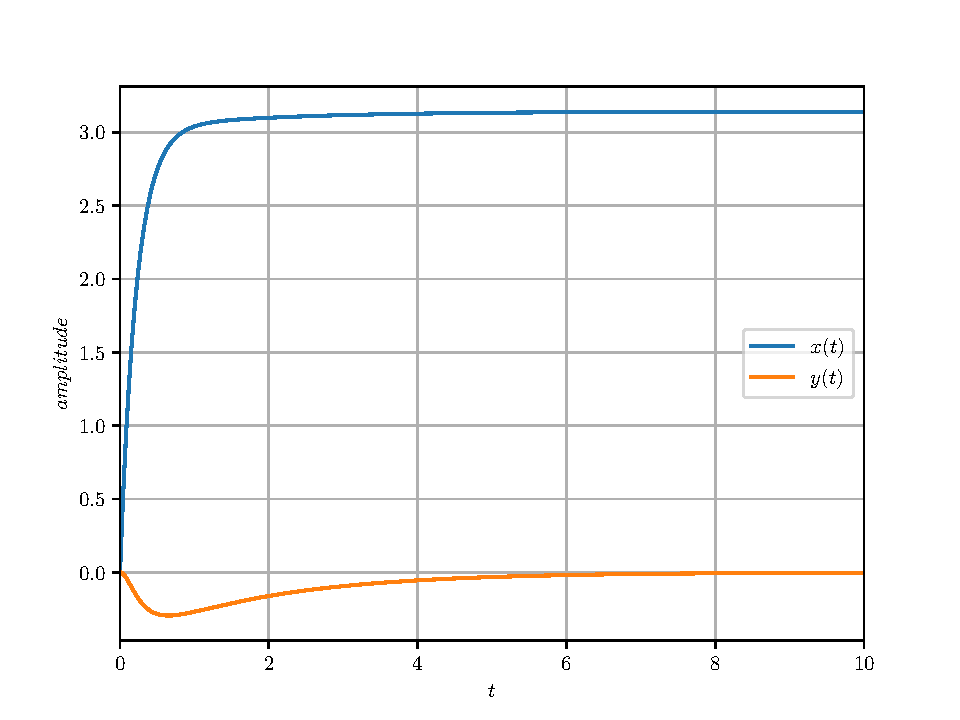
\includegraphics[width=0.9\textwidth]{figures/ex10_invPend35a.pdf}
        \caption{\gr{Χρονική απόκριση ανάστροφου εκκρεμούς,
        \( k = 3.5/a, a = 0.3 \)}}
        \label{fig:ex10_invPend35a}
    \end{figure}
    Στο σχήμα~\ref{fig:ex10_invPend35a} παρουσιάζεται η χρονική απόκριση του
    εκκρεμούς με αρχικές συνθήκες \( (0, 0) \), για μικρή απόσβεση \( a = 0.3 \) και έλεγχο
    \[
        u_1(x) = -\frac{3.5}{a}x + \frac{3.5}{a}\pi.
    \]
    Στην περίπτωση αυτή το σύστημα ισορροπεί πολύ πιο γρήγορα. Δεδομένου ότι στο
    παράδειγμα δεν έχουμε κάποιο δείκτη επίδοσης που να περιορίζει τις τιμές του
    \( k \) είμαστε ελεύθεροι να τις επιλέξουμε όσο μεγάλες επιθυμούμε. Παρόλα
    αυτά μία τιμή του \( k \) σε αυτή την περιοχή φαίνεται αρκετά λογική γιατί
    στην πράξη ο έλεγχος θα είναι πάντα φραγμένος.

    Στο σχήμα~\ref{fig:ex10_invPend35aComb} παρουσιάζεται το πορτρέτο κίνησης
    για \( k = 3.5/a, a = 0.3 \).
    \begin{figure}[h]
        \centering
        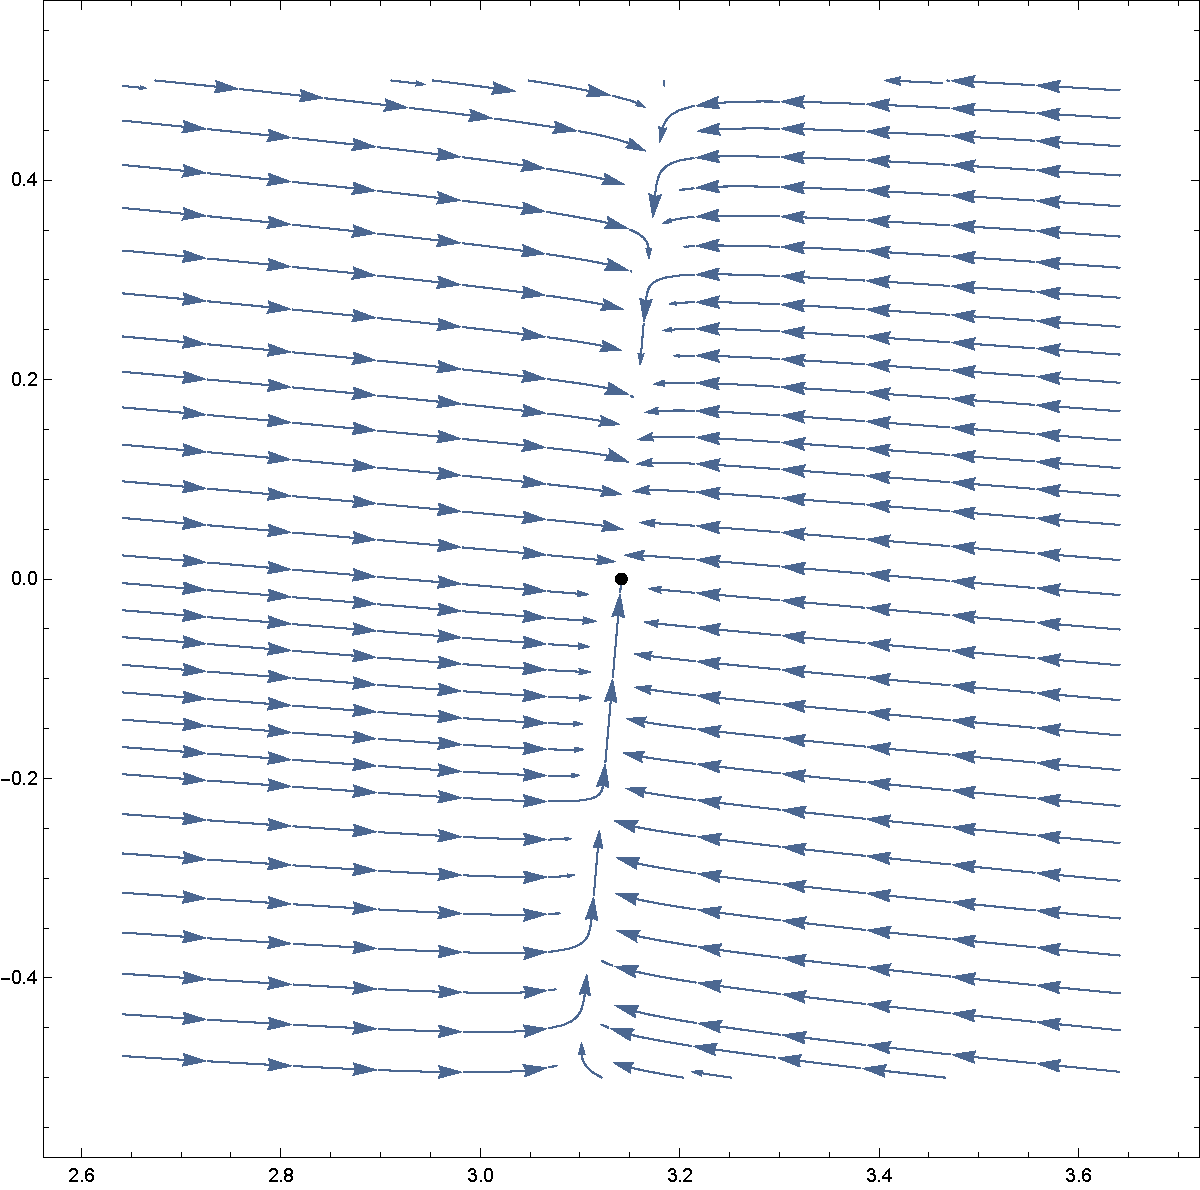
\includegraphics[width=0.8\textwidth]{figures/ex10_invPend35aComb.pdf}
        \caption{\gr{Πορτρέτο κίνησης ανάστροφου εκκρεμούς,
        \( k = 3.5/a, a = 0.3 \)}}
        \label{fig:ex10_invPend35aComb}
    \end{figure}

    (β). Με τον έλεγχο \( u_2(x) \) οι εξισώσεις είναι
    \begin{align*}
        \dot{x} &= y \\
        \dot{y} &= -a y - \sin{x} - kx + c.
    \end{align*}
    Εφόσον θέλουμε το σημείο \( (\pi, 0) \) να είναι ασυμπτωτικά ευσταθές,
    μπορούμε από τη γραμμικοποίηση να βρούμε τις συνθήκες για το \( k \) που θα
    επιτυγχάνει το στόχο αυτόν. Έτσι έχουμε
    \[
        \begin{pmatrix}
            \dot{x} \\
            \dot{y}
        \end{pmatrix} = F(x, y) =
        \begin{pmatrix}
            y -kx + c \\
            -a y - \sin{x}
        \end{pmatrix}.
    \]
    Η γραμμικοποίηση είναι
    \[
        DF(x, y) =
        \begin{pmatrix}
            0 & 1 \\
            -\cos{x} - k & -a
        \end{pmatrix},
    \]
    και στο σημείο \( (\pi, 0) \) έχουμε
    \[
        DF(\pi, 0) =
        \begin{pmatrix}
            0 & 1 \\
            1 - k & -a
        \end{pmatrix}.
    \]
    Εφόσον θέλουμε ασυμπτωτική ευστάθεια, θα πρέπει \(
    \operatorname{Re}(\lambda) < 0 \). Άρα οι ιδιοτιμές είναι
    \begin{align*}
        \det{\begin{pmatrix}
                -\lambda & 1 \\
                1 - k & -a - \lambda
        \end{pmatrix}} &=
        -\lambda)(-a - \lambda) - 1 + k \\
        &= \lambda a + \lambda^2 - 1 + k \\
        &= \lambda^2 + \lambda a - 1 + k.
    \end{align*}
    Η διακρίνουσα της παραπάνω είναι
    \[
        \Delta = a^2 - 4(-1 + k) = a^2 + 4(1 - k).
    \]
    Η ρίζα της διακρίνουσας είναι
    \begin{align*}
        a^2 + 4(1 - k) &= 0 \\
        1 - k &= -\frac{a^2}{4},
    \end{align*}
    που σημαίνει
    \[
        k = 1 + \frac{a^2}{4}.
    \]
    Άρα έχουμε
    \[
        \Delta > 0 \Rightarrow k < 1 + \frac{a^2}{4}, \quad
        \Delta < 0 \Rightarrow k > 1 + \frac{a^2}{4}, \quad
        \Delta = 0 \Rightarrow k = 1 + \frac{a^2}{4}.
    \]
    Οι ιδιοτιμές δίνονται από τη σχέση
    \begin{equation}\label{eq:ex10b_lambda}
        \lambda = \frac{-a \pm\sqrt{a^2 + 4(1 - k)}}{2},
    \end{equation}
    και θα πάρουμε περιπτώσεις για να βρούμε τις συνθήκες για το \( k \).

    Έστω \( \lambda_1 \) η ιδιοτιμή που αντιστοιχεί όταν μπροστά από την
    τετραγωνική ρίζα έχουμε το θετικό πρόσημο και \( \lambda_2 \) η ιδιοτιμή
    που αντιστοιχεί όταν μπροστά από την τετραγωνική ρίζα έχουμε το αρνητικό
    πρόσημο.

    Αν δούμε αρχικά την περίπτωση που \( \Delta > 0 \), τότε προφανώς η \(
    \lambda_2 < 0 \), άρα μένει να κοιτάξουμε την \( \lambda_1 \). Για να είναι
    αυτή αρνητική πρέπει
    \begin{align*}
        -a + \sqrt{a^2 + 4(1 - k)} &< 0 \\
        a^2 + 4(1 - k) < a^2,
    \end{align*}
    που σημαίνει
    \[
        k < 1.
    \]
    Προφανώς η παραπάνω εμπεριέχει την προηγούμενη συνθήκη ώστε η διακρίνουσα να
    είναι θετική. Άρα για \( k < 1 \) το \( (\pi, 0) \) είναι ασυμπτωτικά
    ευσταθές και έχει τη μορφή ευσταθούς κόμβου.

    Όταν \( \Delta < 0 \), κοιτώντας τη σχέση~\eqref{eq:ex10b_lambda}, επειδή το
    πραγματικό μέρος είναι πάντα αρνητικό αυτό σημαίνει ότι το \( (\pi, 0) \) σημείο
    είναι ασυμπτωτικά ευσταθές με μορφή ευσταθούς εστίας.

    Τέλος, όταν \( \Delta = 0 \), έχουμε διπλή ρίζα και ιδιοτιμές \(
    \lambda_{1,2} = -a/2 \) και το \( (\pi, 0) \) σημείο είναι ασυμπτωτικά
    ευσταθές.

    Στο σχήμα~\ref{fig:ex10_b_invPend4a} παρουσιάζεται η χρονική απόκριση του
    εκκρεμούς με αρχικές συνθήκες \( (0, 0) \), για μικρή απόσβεση \( a = 0.3 \)
    και έλεγχο
    \[
        u_2(x) = -4\left(1 + \frac{a^2}{4}\right)x +
        4\left(1 + \frac{a^2}{4}\right)\pi,
    \]
    και στο σχήμα~\ref{fig:ex10_b_invPend4Comb} το αντίστοιχο πορτρέτο κίνησης.
    \begin{figure}[h]
        \centering
        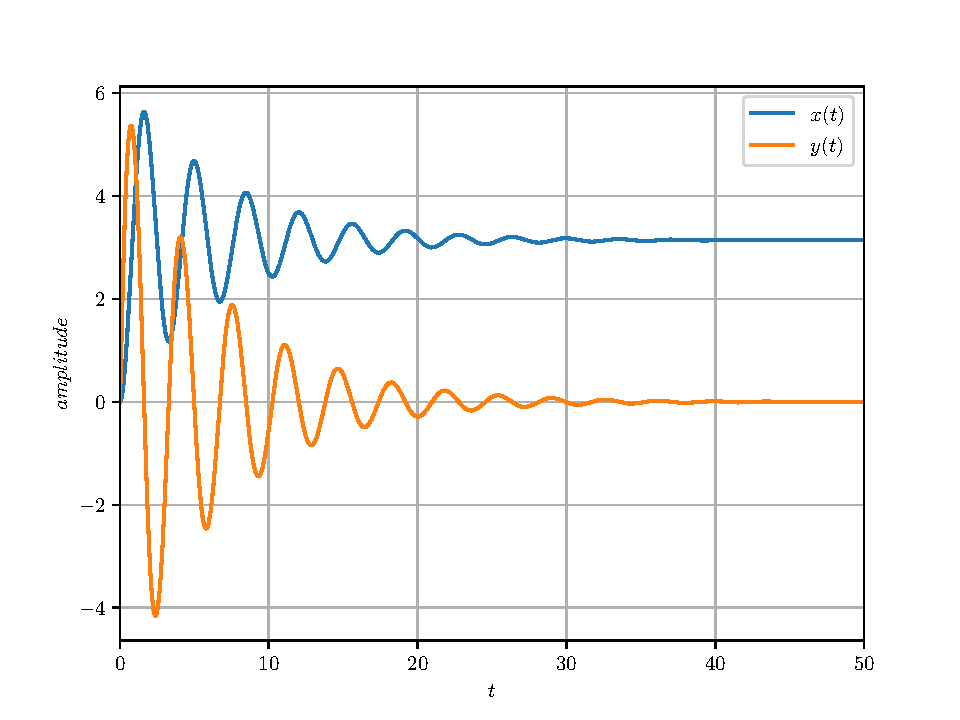
\includegraphics[width=0.9\textwidth]{figures/ex10_b_invPend4a.pdf}
        \caption{\gr{Χρονική απόκριση ανάστροφου εκκρεμούς,
        \( k = 4(1 + a^2/4), a = 0.3 \)}}
        \label{fig:ex10_b_invPend4a}
    \end{figure}
    \begin{figure}[h]
        \centering
        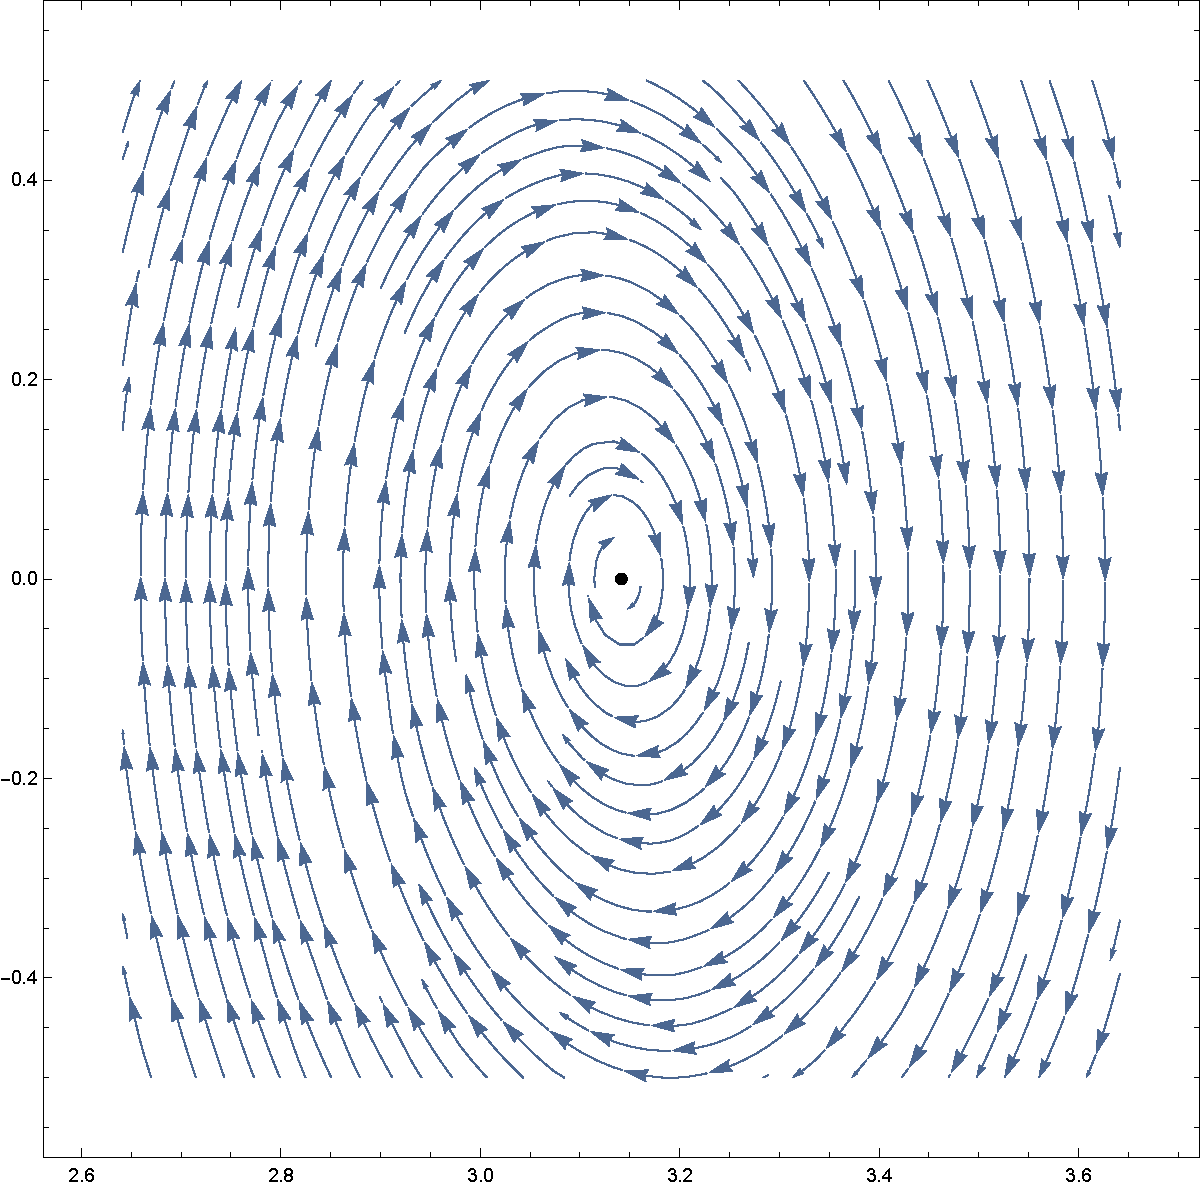
\includegraphics[width=0.8\textwidth]{figures/ex10_b_invPend4Comb.pdf}
        \caption{\gr{Πορτρέτο κίνησης ανάστροφου εκκρεμούς,
        \( k = 4(1 + a^2/4), a = 0.3 \)}}
        \label{fig:ex10_b_invPend4Comb}
    \end{figure}
    Είναι προφανές ότι βρισκόμαστε στην περιοχή της ευσταθής εστίας. Από τα
    διαγράμματα παρατηρούμαι ότι ο στόχος είναι αρκετά δυσκολότερος. Η μικρή
    απόσβεση δημιουργεί μεγάλες ταλαντώσεις στον έλεγχο της ταχύτητας του
    εκκρεμούς. Μεγαλώνοντας το κέρδος \( k \) θα φτάσουμε συντομότερα στο σημείο
    \( (\pi, 0) \), άλλα θα εμφανιστούν ακόμα μεγαλύτερες ταλαντώσεις. Ιδανικά
    θα επιλέγαμε μία απόσβεση με τιμές γύρω στο \( 0.8 - 0.9 \) για καλύτερες
    αποδόσεις.

    Στο σχήμα~\ref{fig:ex10_b_invPendll} παρουσιάζεται η χρονική απόκριση του
    εκκρεμούς με αρχικές συνθήκες \( (0, 0) \), για μικρή απόσβεση \( a = 0.3 \)
    και έλεγχο
    \[
        u_2(x) = -\left(1 + \frac{a^2}{4}\right)x +
        \left(1 + \frac{a^2}{4}\right)\pi,
    \]
    και στο σχήμα~\ref{fig:ex10_b_invPendllComb} το αντίστοιχο πορτρέτο κίνησης.
    \begin{figure}[h]
        \centering
        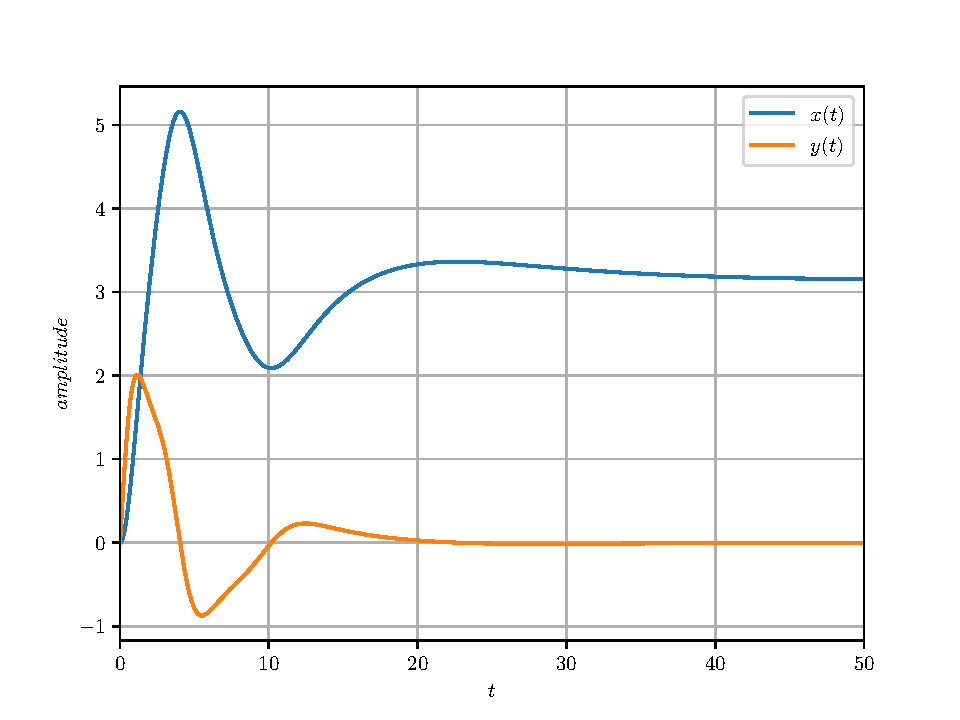
\includegraphics[width=0.9\textwidth]{figures/ex10_b_invPendll.pdf}
        \caption{\gr{Χρονική απόκριση ανάστροφου εκκρεμούς,
        \( k = 1 + a^2/4, a = 0.3 \)}}
        \label{fig:ex10_b_invPendll}
    \end{figure}
    \begin{figure}[h]
        \centering
        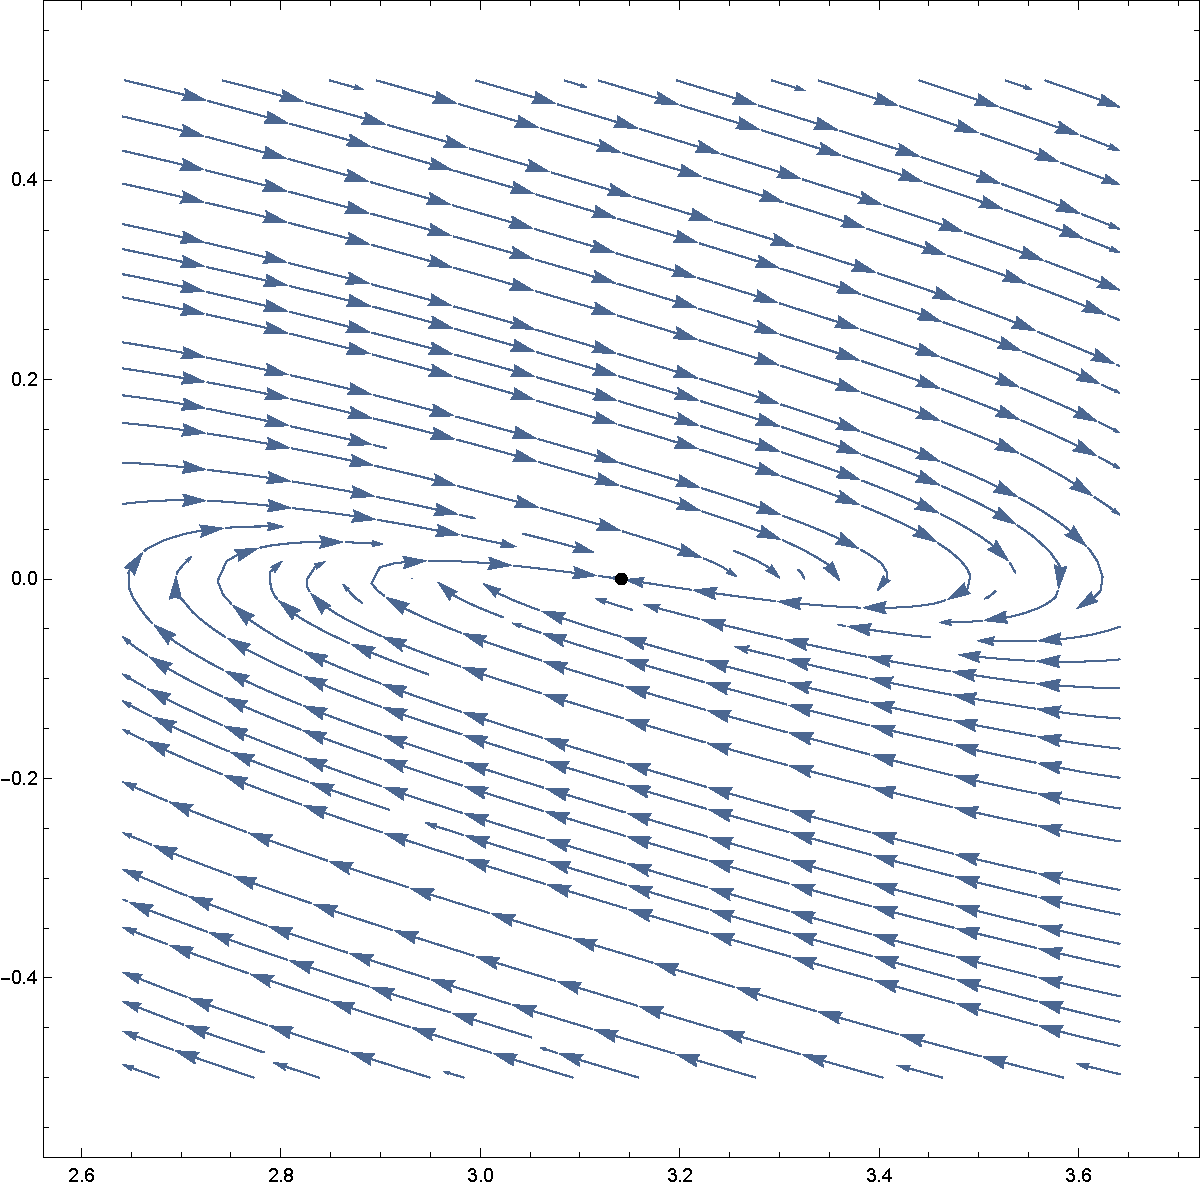
\includegraphics[width=0.8\textwidth]{figures/ex10_b_invPendllComb.pdf}
        \caption{\gr{Πορτρέτο κίνησης ανάστροφου εκκρεμούς,
        \( k = 1 + a^2/4, a = 0.3 \)}}
        \label{fig:ex10_b_invPendllComb}
    \end{figure}
    Το παράδειγμα αυτό παρουσιάζεται απλώς για επιβεβαίωση των υπολογισμών.
    Παρατηρούμε πως το \( (\pi, 0) \) είναι ασυμπτωτικά ευσταθές και έχει τη
    μορφή διπλής ρίζας.
\end{solution}

%\newpage
%\selectlanguage{english}
%\printbibliography[title=\greektext{Βιβλιογραφία}]
\end{document}
